% Created 2025-03-11 Tue 20:04
% Intended LaTeX compiler: xelatex
\documentclass[11pt]{article}
\usepackage{capt-of}
\usepackage{hyperref}
% wrong resolution of image
% https://tex.stackexchange.com/questions/21627/image-from-includegraphics-showing-in-wrong-image-size?rq=1

%%%%%%%%%%%%%%%%%%%%%%%%%%%%%%%%%%%%%%
%% TIPS                                 %%
%%%%%%%%%%%%%%%%%%%%%%%%%%%%%%%%%%%%%%
% \substack{a\\b} for multiple lines text
% \usepackage{expl3}
% \expandafter\def\csname ver@l3regex.sty\endcsname{}
% \usepackage{pkgloader}
\usepackage[utf8]{inputenc}

% nfss error
% \usepackage[B1,T1]{fontenc}
\usepackage{fontspec}

% \usepackage[Emoticons]{ucharclasses}
\newfontfamily\DejaSans{DejaVu Sans}
% \setDefaultTransitions{\DejaSans}{}

% pdfplots will load xolor automatically without option
\usepackage[dvipsnames]{xcolor}

%                                                             ┳┳┓   ┓
%                                                             ┃┃┃┏┓╋┣┓
%                                                             ┛ ┗┗┻┗┛┗
% \usepackage{amsmath} mathtools loads the amsmath
\usepackage{amsmath}
\usepackage{mathtools}

\usepackage{amsthm}
\usepackage{amsbsy}

%\usepackage{commath}

\usepackage{amssymb}

\usepackage{mathrsfs}
%\usepackage{mathabx}
\usepackage{stmaryrd}
\usepackage{empheq}

\usepackage{scalerel}
\usepackage{stackengine}
\usepackage{stackrel}



\usepackage{nicematrix}
\usepackage{tensor}
\usepackage{blkarray}
\usepackage{siunitx}
\usepackage[f]{esvect}

% centering \not on a letter
\usepackage{slashed}
\usepackage[makeroom]{cancel}

%\usepackage{merriweather}
\usepackage{unicode-math}
\setmainfont{TeX Gyre Pagella}
% \setmathfont{STIX}
%\setmathfont{texgyrepagella-math.otf}
%\setmathfont{Libertinus Math}
\setmathfont{Latin Modern Math}

 % \setmathfont[range={\smwhtdiamond,\enclosediamond,\varlrtriangle}]{Latin Modern Math}
\setmathfont[range={\rightrightarrows,\twoheadrightarrow,\leftrightsquigarrow,\triangledown,\vartriangle,\precneq,\succneq,\prec,\succ,\preceq,\succeq,\tieconcat}]{XITS Math}
 \setmathfont[range={\int,\setminus}]{Libertinus Math}
 % \setmathfont[range={\mathalpha}]{TeX Gyre Pagella Math}
%\setmathfont[range={\mitA,\mitB,\mitC,\mitD,\mitE,\mitF,\mitG,\mitH,\mitI,\mitJ,\mitK,\mitL,\mitM,\mitN,\mitO,\mitP,\mitQ,\mitR,\mitS,\mitT,\mitU,\mitV,\mitW,\mitX,\mitY,\mitZ,\mita,\mitb,\mitc,\mitd,\mite,\mitf,\mitg,\miti,\mitj,\mitk,\mitl,\mitm,\mitn,\mito,\mitp,\mitq,\mitr,\mits,\mitt,\mitu,\mitv,\mitw,\mitx,\mity,\mitz}]{TeX Gyre Pagella Math}
% unicode is not good at this!
%\let\nmodels\nvDash

 \usepackage{wasysym}

 % for wide hat
 \DeclareSymbolFont{yhlargesymbols}{OMX}{yhex}{m}{n} \DeclareMathAccent{\what}{\mathord}{yhlargesymbols}{"62}

%                                                               ┏┳┓•┓
%                                                                ┃ ┓┃┏┓
%                                                                ┻ ┗┛┗┗

\usepackage{pgfplots}
\pgfplotsset{compat=1.18}
\usepackage{tikz}
\usepackage{tikz-cd}
\tikzcdset{scale cd/.style={every label/.append style={scale=#1},
    cells={nodes={scale=#1}}}}
% TODO: discard qtree and use forest
% \usepackage{tikz-qtree}
\usepackage{forest}

\usetikzlibrary{arrows,positioning,calc,fadings,decorations,matrix,decorations,shapes.misc}
%setting from geogebra
\definecolor{ccqqqq}{rgb}{0.8,0,0}

%                                                          ┳┳┓•    ┓┓
%                                                          ┃┃┃┓┏┏┏┓┃┃┏┓┏┓┏┓┏┓┓┏┏
%                                                          ┛ ┗┗┛┗┗ ┗┗┗┻┛┗┗ ┗┛┗┻┛
%\usepackage{twemojis}
\usepackage[most]{tcolorbox}
\usepackage{threeparttable}
\usepackage{tabularx}

\usepackage{enumitem}
\usepackage[indLines=false]{algpseudocodex}
\usepackage[]{algorithm2e}
% \SetKwComment{Comment}{/* }{ */}
% \algrenewcommand\algorithmicrequire{\textbf{Input:}}
% \algrenewcommand\algorithmicensure{\textbf{Output:}}
% wrong with preview
\usepackage{subcaption}
\usepackage{caption}
% {\aunclfamily\Huge}
\usepackage{auncial}

\usepackage{float}

\usepackage{fancyhdr}

\usepackage{ifthen}
\usepackage{xargs}

\definecolor{mintedbg}{rgb}{0.99,0.99,0.99}
\usepackage[cachedir=\detokenize{~/miscellaneous/trash}]{minted}
\setminted{breaklines,
  mathescape,
  bgcolor=mintedbg,
  fontsize=\footnotesize,
  frame=single,
  linenos}
\usemintedstyle{xcode}
\usepackage{tcolorbox}
\usepackage{etoolbox}



\usepackage{imakeidx}
\usepackage{hyperref}
\usepackage{soul}
\usepackage{framed}

% don't use this for preview
%\usepackage[margin=1.5in]{geometry}
% \usepackage{geometry}
% \geometry{legalpaper, landscape, margin=1in}
\usepackage[font=itshape]{quoting}

%\LoadPackagesNow
%\usepackage[xetex]{preview}
%%%%%%%%%%%%%%%%%%%%%%%%%%%%%%%%%%%%%%%
%% USEPACKAGES end                       %%
%%%%%%%%%%%%%%%%%%%%%%%%%%%%%%%%%%%%%%%

%%%%%%%%%%%%%%%%%%%%%%%%%%%%%%%%%%%%%%%
%% Algorithm environment
%%%%%%%%%%%%%%%%%%%%%%%%%%%%%%%%%%%%%%%
\SetKwIF{Recv}{}{}{upon receiving}{do}{}{}{}
\SetKwBlock{Init}{initially do}{}
\SetKwProg{Function}{Function}{:}{}

% https://github.com/chrmatt/algpseudocodex/issues/3
\algnewcommand\algorithmicswitch{\textbf{switch}}%
\algnewcommand\algorithmiccase{\textbf{case}}
\algnewcommand\algorithmicof{\textbf{of}}
\algnewcommand\algorithmicotherwise{\texttt{otherwise} $\Rightarrow$}

\makeatletter
\algdef{SE}[SWITCH]{Switch}{EndSwitch}[1]{\algpx@startIndent\algpx@startCodeCommand\algorithmicswitch\ #1\ \algorithmicdo}{\algpx@endIndent\algpx@startCodeCommand\algorithmicend\ \algorithmicswitch}%
\algdef{SE}[CASE]{Case}{EndCase}[1]{\algpx@startIndent\algpx@startCodeCommand\algorithmiccase\ #1}{\algpx@endIndent\algpx@startCodeCommand\algorithmicend\ \algorithmiccase}%
\algdef{SE}[CASEOF]{CaseOf}{EndCaseOf}[1]{\algpx@startIndent\algpx@startCodeCommand\algorithmiccase\ #1 \algorithmicof}{\algpx@endIndent\algpx@startCodeCommand\algorithmicend\ \algorithmiccase}
\algdef{SE}[OTHERWISE]{Otherwise}{EndOtherwise}[0]{\algpx@startIndent\algpx@startCodeCommand\algorithmicotherwise}{\algpx@endIndent\algpx@startCodeCommand\algorithmicend\ \algorithmicotherwise}
\ifbool{algpx@noEnd}{%
  \algtext*{EndSwitch}%
  \algtext*{EndCase}%
  \algtext*{EndCaseOf}
  \algtext*{EndOtherwise}
  %
  % end indent line after (not before), to get correct y position for multiline text in last command
  \apptocmd{\EndSwitch}{\algpx@endIndent}{}{}%
  \apptocmd{\EndCase}{\algpx@endIndent}{}{}%
  \apptocmd{\EndCaseOf}{\algpx@endIndent}{}{}
  \apptocmd{\EndOtherwise}{\algpx@endIndent}{}{}
}{}%

\pretocmd{\Switch}{\algpx@endCodeCommand}{}{}
\pretocmd{\Case}{\algpx@endCodeCommand}{}{}
\pretocmd{\CaseOf}{\algpx@endCodeCommand}{}{}
\pretocmd{\Otherwise}{\algpx@endCodeCommand}{}{}

% for end commands that may not be printed, tell endCodeCommand whether we are using noEnd
\ifbool{algpx@noEnd}{%
  \pretocmd{\EndSwitch}{\algpx@endCodeCommand[1]}{}{}%
  \pretocmd{\EndCase}{\algpx@endCodeCommand[1]}{}{}
  \pretocmd{\EndCaseOf}{\algpx@endCodeCommand[1]}{}{}%
  \pretocmd{\EndOtherwise}{\algpx@endCodeCommand[1]}{}{}
}{%
  \pretocmd{\EndSwitch}{\algpx@endCodeCommand[0]}{}{}%
  \pretocmd{\EndCase}{\algpx@endCodeCommand[0]}{}{}%
  \pretocmd{\EndCaseOf}{\algpx@endCodeCommand[0]}{}{}
  \pretocmd{\EndOtherwise}{\algpx@endCodeCommand[0]}{}{}
}%
\makeatother
% % For algpseudocode
% \algnewcommand\algorithmicswitch{\textbf{switch}}
% \algnewcommand\algorithmiccase{\textbf{case}}
% \algnewcommand\algorithmiccaseof{\textbf{case}}
% \algnewcommand\algorithmicof{\textbf{of}}
% % New "environments"
% \algdef{SE}[SWITCH]{Switch}{EndSwitch}[1]{\algorithmicswitch\ #1\ \algorithmicdo}{\algorithmicend\ \algorithmicswitch}%
% \algdef{SE}[CASE]{Case}{EndCase}[1]{\algorithmiccase\ #1}{\algorithmicend\ \algorithmiccase}%
% \algtext*{EndSwitch}%
% \algtext*{EndCase}
% \algdef{SE}[CASEOF]{CaseOf}{EndCaseOf}[1]{\algorithmiccaseof\ #1 \algorithmicof}{\algorithmicend\ \algorithmiccaseof}
% \algtext*{EndCaseOf}



%\pdfcompresslevel0

% quoting from
% https://tex.stackexchange.com/questions/391726/the-quotation-environment
\NewDocumentCommand{\bywhom}{m}{% the Bourbaki trick
  {\nobreak\hfill\penalty50\hskip1em\null\nobreak
   \hfill\mbox{\normalfont(#1)}%
   \parfillskip=0pt \finalhyphendemerits=0 \par}%
}

\NewDocumentEnvironment{pquotation}{m}
  {\begin{quoting}[
     indentfirst=true,
     leftmargin=\parindent,
     rightmargin=\parindent]\itshape}
  {\bywhom{#1}\end{quoting}}

\indexsetup{othercode=\small}
\makeindex[columns=2,options={-s /media/wu/file/stuuudy/notes/index_style.ist},intoc]
\makeatletter
\def\@idxitem{\par\hangindent 0pt}
\makeatother


% \newcounter{dummy} \numberwithin{dummy}{section}
\newtheorem{dummy}{dummy}[section]
\theoremstyle{definition}
\newtheorem{definition}[dummy]{Definition}
\theoremstyle{plain}
\newtheorem{corollary}[dummy]{Corollary}
\newtheorem{lemma}[dummy]{Lemma}
\newtheorem{proposition}[dummy]{Proposition}
\newtheorem{theorem}[dummy]{Theorem}
\newtheorem{notation}[dummy]{Notation}
\newtheorem{conjecture}[dummy]{Conjecture}
\newtheorem{fact}[dummy]{Fact}
\newtheorem{warning}[dummy]{Warning}
\theoremstyle{definition}
\newtheorem{examplle}{Example}[section]
\theoremstyle{remark}
\newtheorem*{remark}{Remark}
\newtheorem{exercise}{Exercise}[subsection]
\newtheorem{problem}{Problem}[subsection]
\newtheorem{observation}{Observation}[section]
\newenvironment{claim}[1]{\par\noindent\textbf{Claim:}\space#1}{}

\makeatletter
\DeclareFontFamily{U}{tipa}{}
\DeclareFontShape{U}{tipa}{m}{n}{<->tipa10}{}
\newcommand{\arc@char}{{\usefont{U}{tipa}{m}{n}\symbol{62}}}%

\newcommand{\arc}[1]{\mathpalette\arc@arc{#1}}

\newcommand{\arc@arc}[2]{%
  \sbox0{$\m@th#1#2$}%
  \vbox{
    \hbox{\resizebox{\wd0}{\height}{\arc@char}}
    \nointerlineskip
    \box0
  }%
}
\makeatother

\setcounter{MaxMatrixCols}{20}
%%%%%%% ABS
\DeclarePairedDelimiter\abss{\lvert}{\rvert}%
\DeclarePairedDelimiter\normm{\lVert}{\rVert}%

% Swap the definition of \abs* and \norm*, so that \abs
% and \norm resizes the size of the brackets, and the
% starred version does not.
\makeatletter
\let\oldabs\abss
%\def\abs{\@ifstar{\oldabs}{\oldabs*}}
\newcommand{\abs}{\@ifstar{\oldabs}{\oldabs*}}
\newcommand{\norm}[1]{\left\lVert#1\right\rVert}
%\let\oldnorm\normm
%\def\norm{\@ifstar{\oldnorm}{\oldnorm*}}
%\renewcommand{norm}{\@ifstar{\oldnorm}{\oldnorm*}}
\makeatother

% \stackMath
% \newcommand\what[1]{%
% \savestack{\tmpbox}{\stretchto{%
%   \scaleto{%
%     \scalerel*[\widthof{\ensuremath{#1}}]{\kern-.6pt\bigwedge\kern-.6pt}%
%     {\rule[-\textheight/2]{1ex}{\textheight}}%WIDTH-LIMITED BIG WEDGE
%   }{\textheight}%
% }{0.5ex}}%
% \stackon[1pt]{#1}{\tmpbox}%
% }

% \newcommand\what[1]{\ThisStyle{%
%     \setbox0=\hbox{$\SavedStyle#1$}%
%     \stackengine{-1.0\ht0+.5pt}{$\SavedStyle#1$}{%
%       \stretchto{\scaleto{\SavedStyle\mkern.15mu\char'136}{2.6\wd0}}{1.4\ht0}%
%     }{O}{c}{F}{T}{S}%
%   }
% }

% \newcommand\wtilde[1]{\ThisStyle{%
%     \setbox0=\hbox{$\SavedStyle#1$}%
%     \stackengine{-.1\LMpt}{$\SavedStyle#1$}{%
%       \stretchto{\scaleto{\SavedStyle\mkern.2mu\AC}{.5150\wd0}}{.6\ht0}%
%     }{O}{c}{F}{T}{S}%
%   }
% }

% \newcommand\wbar[1]{\ThisStyle{%
%     \setbox0=\hbox{$\SavedStyle#1$}%
%     \stackengine{.5pt+\LMpt}{$\SavedStyle#1$}{%
%       \rule{\wd0}{\dimexpr.3\LMpt+.3pt}%
%     }{O}{c}{F}{T}{S}%
%   }
% }

\newcommand{\bl}[1] {\boldsymbol{#1}}
\newcommand{\Wt}[1] {\stackrel{\sim}{\smash{#1}\rule{0pt}{1.1ex}}}
\newcommand{\wt}[1] {\widetilde{#1}}
\newcommand{\tf}[1] {\textbf{#1}}

\newcommand{\wu}[1]{{\color{red} #1}}

%For boxed texts in align, use Aboxed{}
%otherwise use boxed{}

\DeclareMathSymbol{\widehatsym}{\mathord}{largesymbols}{"62}
\newcommand\lowerwidehatsym{%
  \text{\smash{\raisebox{-1.3ex}{%
    $\widehatsym$}}}}
\newcommand\fixwidehat[1]{%
  \mathchoice
    {\accentset{\displaystyle\lowerwidehatsym}{#1}}
    {\accentset{\textstyle\lowerwidehatsym}{#1}}
    {\accentset{\scriptstyle\lowerwidehatsym}{#1}}
    {\accentset{\scriptscriptstyle\lowerwidehatsym}{#1}}
  }


\newcommand{\cupdot}{\mathbin{\dot{\cup}}}
\newcommand{\bigcupdot}{\mathop{\dot{\bigcup}}}

\usepackage{graphicx}

\usepackage[toc,page]{appendix}

% text on arrow for xRightarrow
\makeatletter
%\newcommand{\xRightarrow}[2][]{\ext@arrow 0359\Rightarrowfill@{#1}{#2}}
\makeatother

% Arbitrary long arrow
\newcommand{\Rarrow}[1]{%
\parbox{#1}{\tikz{\draw[->](0,0)--(#1,0);}}
}

\newcommand{\LRarrow}[1]{%
\parbox{#1}{\tikz{\draw[<->](0,0)--(#1,0);}}
}


\makeatletter
\providecommand*{\rmodels}{%
  \mathrel{%
    \mathpalette\@rmodels\models
  }%
}
\newcommand*{\@rmodels}[2]{%
  \reflectbox{$\m@th#1#2$}%
}
\makeatother

% Roman numerals
\makeatletter
\newcommand*{\rom}[1]{\expandafter\@slowromancap\romannumeral #1@}
\makeatother
% \\def \\b\([a-zA-Z]\) {\\boldsymbol{[a-zA-z]}}
% \\DeclareMathOperator{\\b\1}{\\textbf{\1}}

\DeclareMathOperator*{\argmin}{arg\,min}
\DeclareMathOperator*{\argmax}{arg\,max}

\DeclareMathOperator{\bone}{\textbf{1}}
\DeclareMathOperator{\bx}{\textbf{x}}
\DeclareMathOperator{\bz}{\textbf{z}}
\DeclareMathOperator{\bff}{\textbf{f}}
\DeclareMathOperator{\ba}{\textbf{a}}
\DeclareMathOperator{\bk}{\textbf{k}}
\DeclareMathOperator{\bs}{\textbf{s}}
\DeclareMathOperator{\bh}{\textbf{h}}
\DeclareMathOperator{\bc}{\textbf{c}}
\DeclareMathOperator{\br}{\textbf{r}}
\DeclareMathOperator{\bi}{\textbf{i}}
\DeclareMathOperator{\bj}{\textbf{j}}
\DeclareMathOperator{\bn}{\textbf{n}}
\DeclareMathOperator{\be}{\textbf{e}}
\DeclareMathOperator{\bo}{\textbf{o}}
\DeclareMathOperator{\bU}{\textbf{U}}
\DeclareMathOperator{\bL}{\textbf{L}}
\DeclareMathOperator{\bV}{\textbf{V}}
\def \bzero {\mathbf{0}}
\def \bbone {\mathbb{1}}
\def \btwo {\mathbf{2}}
\DeclareMathOperator{\bv}{\textbf{v}}
\DeclareMathOperator{\bp}{\textbf{p}}
\DeclareMathOperator{\bI}{\textbf{I}}
\def \dbI {\dot{\bI}}
\DeclareMathOperator{\bM}{\textbf{M}}
\DeclareMathOperator{\bN}{\textbf{N}}
\DeclareMathOperator{\bK}{\textbf{K}}
\DeclareMathOperator{\bt}{\textbf{t}}
\DeclareMathOperator{\bb}{\textbf{b}}
\DeclareMathOperator{\bA}{\textbf{A}}
\DeclareMathOperator{\bX}{\textbf{X}}
\DeclareMathOperator{\bu}{\textbf{u}}
\DeclareMathOperator{\bS}{\textbf{S}}
\DeclareMathOperator{\bZ}{\textbf{Z}}
\DeclareMathOperator{\bJ}{\textbf{J}}
\DeclareMathOperator{\by}{\textbf{y}}
\DeclareMathOperator{\bw}{\textbf{w}}
\DeclareMathOperator{\bT}{\textbf{T}}
\DeclareMathOperator{\bF}{\textbf{F}}
\DeclareMathOperator{\bmm}{\textbf{m}}
\DeclareMathOperator{\bW}{\textbf{W}}
\DeclareMathOperator{\bR}{\textbf{R}}
\DeclareMathOperator{\bC}{\textbf{C}}
\DeclareMathOperator{\bD}{\textbf{D}}
\DeclareMathOperator{\bE}{\textbf{E}}
\DeclareMathOperator{\bQ}{\textbf{Q}}
\DeclareMathOperator{\bP}{\textbf{P}}
\DeclareMathOperator{\bY}{\textbf{Y}}
\DeclareMathOperator{\bH}{\textbf{H}}
\DeclareMathOperator{\bB}{\textbf{B}}
\DeclareMathOperator{\bG}{\textbf{G}}
\def \blambda {\symbf{\lambda}}
\def \boldeta {\symbf{\eta}}
\def \balpha {\symbf{\alpha}}
\def \btau {\symbf{\tau}}
\def \bbeta {\symbf{\beta}}
\def \bgamma {\symbf{\gamma}}
\def \bxi {\symbf{\xi}}
\def \bLambda {\symbf{\Lambda}}
\def \bGamma {\symbf{\Gamma}}

\newcommand{\bto}{{\boldsymbol{\to}}}
\newcommand{\Ra}{\Rightarrow}
\newcommand{\xrsa}[1]{\overset{#1}{\rightsquigarrow}}
\newcommand{\xlsa}[1]{\overset{#1}{\leftsquigarrow}}
\newcommand\und[1]{\underline{#1}}
\newcommand\ove[1]{\overline{#1}}
%\def \concat {\verb|^|}
\def \bPhi {\mbfPhi}
\def \btheta {\mbftheta}
\def \bTheta {\mbfTheta}
\def \bmu {\mbfmu}
\def \bphi {\mbfphi}
\def \bSigma {\mbfSigma}
\def \la {\langle}
\def \ra {\rangle}

\def \caln {\mathcal{N}}
\def \dissum {\displaystyle\Sigma}
\def \dispro {\displaystyle\prod}

\def \caret {\verb!^!}

\def \A {\mathbb{A}}
\def \B {\mathbb{B}}
\def \C {\mathbb{C}}
\def \D {\mathbb{D}}
\def \E {\mathbb{E}}
\def \F {\mathbb{F}}
\def \G {\mathbb{G}}
\def \H {\mathbb{H}}
\def \I {\mathbb{I}}
\def \J {\mathbb{J}}
\def \K {\mathbb{K}}
\def \L {\mathbb{L}}
\def \M {\mathbb{M}}
\def \N {\mathbb{N}}
\def \O {\mathbb{O}}
\def \P {\mathbb{P}}
\def \Q {\mathbb{Q}}
\def \R {\mathbb{R}}
\def \S {\mathbb{S}}
\def \T {\mathbb{T}}
\def \U {\mathbb{U}}
\def \V {\mathbb{V}}
\def \W {\mathbb{W}}
\def \X {\mathbb{X}}
\def \Y {\mathbb{Y}}
\def \Z {\mathbb{Z}}

\def \cala {\mathcal{A}}
\def \cale {\mathcal{E}}
\def \calb {\mathcal{B}}
\def \calq {\mathcal{Q}}
\def \calp {\mathcal{P}}
\def \cals {\mathcal{S}}
\def \calx {\mathcal{X}}
\def \caly {\mathcal{Y}}
\def \calg {\mathcal{G}}
\def \cald {\mathcal{D}}
\def \caln {\mathcal{N}}
\def \calr {\mathcal{R}}
\def \calt {\mathcal{T}}
\def \calm {\mathcal{M}}
\def \calw {\mathcal{W}}
\def \calc {\mathcal{C}}
\def \calv {\mathcal{V}}
\def \calf {\mathcal{F}}
\def \calk {\mathcal{K}}
\def \call {\mathcal{L}}
\def \calu {\mathcal{U}}
\def \calo {\mathcal{O}}
\def \calh {\mathcal{H}}
\def \cali {\mathcal{I}}
\def \calj {\mathcal{J}}

\def \bcup {\bigcup}

% set theory

\def \zfcc {\textbf{ZFC}^-}
\def \BGC {\textbf{BGC}}
\def \BG {\textbf{BG}}
\def \ac  {\textbf{AC}}
\def \gl  {\textbf{L }}
\def \gll {\textbf{L}}
\newcommand{\zfm}{$\textbf{ZF}^-$}

\def \ZFm {\text{ZF}^-}
\def \ZFCm {\text{ZFC}^-}
\DeclareMathOperator{\WF}{WF}
\DeclareMathOperator{\On}{On}
\def \on {\textbf{On }}
\def \cm {\textbf{M }}
\def \cn {\textbf{N }}
\def \cv {\textbf{V }}
\def \zc {\textbf{ZC }}
\def \zcm {\textbf{ZC}}
\def \zff {\textbf{ZF}}
\def \wfm {\textbf{WF}}
\def \onm {\textbf{On}}
\def \cmm {\textbf{M}}
\def \cnm {\textbf{N}}
\def \cvm {\textbf{V}}

\renewcommand{\restriction}{\mathord{\upharpoonright}}
%% another restriction
\newcommand\restr[2]{{% we make the whole thing an ordinary symbol
  \left.\kern-\nulldelimiterspace % automatically resize the bar with \right
  #1 % the function
  \vphantom{\big|} % pretend it's a little taller at normal size
  \right|_{#2} % this is the delimiter
  }}

\def \pred {\text{pred}}

\def \rank {\text{rank}}
\def \Con {\text{Con}}
\def \deff {\text{Def}}


\def \uin {\underline{\in}}
\def \oin {\overline{\in}}
\def \uR {\underline{R}}
\def \oR {\overline{R}}
\def \uP {\underline{P}}
\def \oP {\overline{P}}

\def \dsum {\displaystyle\sum}

\def \Ra {\Rightarrow}

\def \e {\enspace}

\def \sgn {\operatorname{sgn}}
\def \gen {\operatorname{gen}}
\def \Hom {\operatorname{Hom}}
\def \hom {\operatorname{hom}}
\def \Sub {\operatorname{Sub}}

\def \supp {\operatorname{supp}}

\def \epiarrow {\twoheadarrow}
\def \monoarrow {\rightarrowtail}
\def \rrarrow {\rightrightarrows}

% \def \minus {\text{-}}
% \newcommand{\minus}{\scalebox{0.75}[1.0]{$-$}}
% \DeclareUnicodeCharacter{002D}{\minus}


\def \tril {\triangleleft}

\def \ISigma {\text{I}\Sigma}
\def \IDelta {\text{I}\Delta}
\def \IPi {\text{I}\Pi}
\def \ACF {\textsf{ACF}}
\def \pCF {\textit{p}\text{CF}}
\def \ACVF {\textsf{ACVF}}
\def \HLR {\textsf{HLR}}
\def \OAG {\textsf{OAG}}
\def \RCF {\textsf{RCF}}
\DeclareMathOperator{\GL}{GL}
\DeclareMathOperator{\PGL}{PGL}
\DeclareMathOperator{\SL}{SL}
\DeclareMathOperator{\Inv}{Inv}
\DeclareMathOperator{\res}{res}
\DeclareMathOperator{\Sym}{Sym}
%\DeclareMathOperator{\char}{char}
\def \equal {=}

\def \degree {\text{degree}}
\def \app {\text{App}}
\def \FV {\text{FV}}
\def \conv {\text{conv}}
\def \cont {\text{cont}}
\DeclareMathOperator{\cl}{\text{cl}}
\DeclareMathOperator{\trcl}{\text{trcl}}
\DeclareMathOperator{\sg}{sg}
\DeclareMathOperator{\trdeg}{trdeg}
\def \Ord {\text{Ord}}

\DeclareMathOperator{\cf}{cf}
\DeclareMathOperator{\zfc}{ZFC}

%\DeclareMathOperator{\Th}{Th}
%\def \th {\text{Th}}
% \newcommand{\th}{\text{Th}}
\DeclareMathOperator{\type}{type}
\DeclareMathOperator{\zf}{\textbf{ZF}}
\def \fa {\mathfrak{a}}
\def \fb {\mathfrak{b}}
\def \fc {\mathfrak{c}}
\def \fd {\mathfrak{d}}
\def \fe {\mathfrak{e}}
\def \ff {\mathfrak{f}}
\def \fg {\mathfrak{g}}
\def \fh {\mathfrak{h}}
%\def \fi {\mathfrak{i}}
\def \fj {\mathfrak{j}}
\def \fk {\mathfrak{k}}
\def \fl {\mathfrak{l}}
\def \fm {\mathfrak{m}}
\def \fn {\mathfrak{n}}
\def \fo {\mathfrak{o}}
\def \fp {\mathfrak{p}}
\def \fq {\mathfrak{q}}
\def \fr {\mathfrak{r}}
\def \fs {\mathfrak{s}}
\def \ft {\mathfrak{t}}
\def \fu {\mathfrak{u}}
\def \fv {\mathfrak{v}}
\def \fw {\mathfrak{w}}
\def \fx {\mathfrak{x}}
\def \fy {\mathfrak{y}}
\def \fz {\mathfrak{z}}
\def \fA {\mathfrak{A}}
\def \fB {\mathfrak{B}}
\def \fC {\mathfrak{C}}
\def \fD {\mathfrak{D}}
\def \fE {\mathfrak{E}}
\def \fF {\mathfrak{F}}
\def \fG {\mathfrak{G}}
\def \fH {\mathfrak{H}}
\def \fI {\mathfrak{I}}
\def \fJ {\mathfrak{J}}
\def \fK {\mathfrak{K}}
\def \fL {\mathfrak{L}}
\def \fM {\mathfrak{M}}
\def \fN {\mathfrak{N}}
\def \fO {\mathfrak{O}}
\def \fP {\mathfrak{P}}
\def \fQ {\mathfrak{Q}}
\def \fR {\mathfrak{R}}
\def \fS {\mathfrak{S}}
\def \fT {\mathfrak{T}}
\def \fU {\mathfrak{U}}
\def \fV {\mathfrak{V}}
\def \fW {\mathfrak{W}}
\def \fX {\mathfrak{X}}
\def \fY {\mathfrak{Y}}
\def \fZ {\mathfrak{Z}}

\def \sfA {\textsf{A}}
\def \sfB {\textsf{B}}
\def \sfC {\textsf{C}}
\def \sfD {\textsf{D}}
\def \sfE {\textsf{E}}
\def \sfF {\textsf{F}}
\def \sfG {\textsf{G}}
\def \sfH {\textsf{H}}
\def \sfI {\textsf{I}}
\def \sfJ {\textsf{J}}
\def \sfK {\textsf{K}}
\def \sfL {\textsf{L}}
\def \sfM {\textsf{M}}
\def \sfN {\textsf{N}}
\def \sfO {\textsf{O}}
\def \sfP {\textsf{P}}
\def \sfQ {\textsf{Q}}
\def \sfR {\textsf{R}}
\def \sfS {\textsf{S}}
\def \sfT {\textsf{T}}
\def \sfU {\textsf{U}}
\def \sfV {\textsf{V}}
\def \sfW {\textsf{W}}
\def \sfX {\textsf{X}}
\def \sfY {\textsf{Y}}
\def \sfZ {\textsf{Z}}
\def \sfa {\textsf{a}}
\def \sfb {\textsf{b}}
\def \sfc {\textsf{c}}
\def \sfd {\textsf{d}}
\def \sfe {\textsf{e}}
\def \sff {\textsf{f}}
\def \sfg {\textsf{g}}
\def \sfh {\textsf{h}}
\def \sfi {\textsf{i}}
\def \sfj {\textsf{j}}
\def \sfk {\textsf{k}}
\def \sfl {\textsf{l}}
\def \sfm {\textsf{m}}
\def \sfn {\textsf{n}}
\def \sfo {\textsf{o}}
\def \sfp {\textsf{p}}
\def \sfq {\textsf{q}}
\def \sfr {\textsf{r}}
\def \sfs {\textsf{s}}
\def \sft {\textsf{t}}
\def \sfu {\textsf{u}}
\def \sfv {\textsf{v}}
\def \sfw {\textsf{w}}
\def \sfx {\textsf{x}}
\def \sfy {\textsf{y}}
\def \sfz {\textsf{z}}

\def \ttA {\texttt{A}}
\def \ttB {\texttt{B}}
\def \ttC {\texttt{C}}
\def \ttD {\texttt{D}}
\def \ttE {\texttt{E}}
\def \ttF {\texttt{F}}
\def \ttG {\texttt{G}}
\def \ttH {\texttt{H}}
\def \ttI {\texttt{I}}
\def \ttJ {\texttt{J}}
\def \ttK {\texttt{K}}
\def \ttL {\texttt{L}}
\def \ttM {\texttt{M}}
\def \ttN {\texttt{N}}
\def \ttO {\texttt{O}}
\def \ttP {\texttt{P}}
\def \ttQ {\texttt{Q}}
\def \ttR {\texttt{R}}
\def \ttS {\texttt{S}}
\def \ttT {\texttt{T}}
\def \ttU {\texttt{U}}
\def \ttV {\texttt{V}}
\def \ttW {\texttt{W}}
\def \ttX {\texttt{X}}
\def \ttY {\texttt{Y}}
\def \ttZ {\texttt{Z}}
\def \tta {\texttt{a}}
\def \ttb {\texttt{b}}
\def \ttc {\texttt{c}}
\def \ttd {\texttt{d}}
\def \tte {\texttt{e}}
\def \ttf {\texttt{f}}
\def \ttg {\texttt{g}}
\def \tth {\texttt{h}}
\def \tti {\texttt{i}}
\def \ttj {\texttt{j}}
\def \ttk {\texttt{k}}
\def \ttl {\texttt{l}}
\def \ttm {\texttt{m}}
\def \ttn {\texttt{n}}
\def \tto {\texttt{o}}
\def \ttp {\texttt{p}}
\def \ttq {\texttt{q}}
\def \ttr {\texttt{r}}
\def \tts {\texttt{s}}
\def \ttt {\texttt{t}}
\def \ttu {\texttt{u}}
\def \ttv {\texttt{v}}
\def \ttw {\texttt{w}}
\def \ttx {\texttt{x}}
\def \tty {\texttt{y}}
\def \ttz {\texttt{z}}

\def \bara {\bbar{a}}
\def \barb {\bbar{b}}
\def \barc {\bbar{c}}
\def \bard {\bbar{d}}
\def \bare {\bbar{e}}
\def \barf {\bbar{f}}
\def \barg {\bbar{g}}
\def \barh {\bbar{h}}
\def \bari {\bbar{i}}
\def \barj {\bbar{j}}
\def \bark {\bbar{k}}
\def \barl {\bbar{l}}
\def \barm {\bbar{m}}
\def \barn {\bbar{n}}
\def \baro {\bbar{o}}
\def \barp {\bbar{p}}
\def \barq {\bbar{q}}
\def \barr {\bbar{r}}
\def \bars {\bbar{s}}
\def \bart {\bbar{t}}
\def \baru {\bbar{u}}
\def \barv {\bbar{v}}
\def \barw {\bbar{w}}
\def \barx {\bbar{x}}
\def \bary {\bbar{y}}
\def \barz {\bbar{z}}
\def \barA {\bbar{A}}
\def \barB {\bbar{B}}
\def \barC {\bbar{C}}
\def \barD {\bbar{D}}
\def \barE {\bbar{E}}
\def \barF {\bbar{F}}
\def \barG {\bbar{G}}
\def \barH {\bbar{H}}
\def \barI {\bbar{I}}
\def \barJ {\bbar{J}}
\def \barK {\bbar{K}}
\def \barL {\bbar{L}}
\def \barM {\bbar{M}}
\def \barN {\bbar{N}}
\def \barO {\bbar{O}}
\def \barP {\bbar{P}}
\def \barQ {\bbar{Q}}
\def \barR {\bbar{R}}
\def \barS {\bbar{S}}
\def \barT {\bbar{T}}
\def \barU {\bbar{U}}
\def \barVV {\bbar{V}}
\def \barW {\bbar{W}}
\def \barX {\bbar{X}}
\def \barY {\bbar{Y}}
\def \barZ {\bbar{Z}}

\def \baralpha {\bbar{\alpha}}
\def \bartau {\bbar{\tau}}
\def \barsigma {\bbar{\sigma}}
\def \barzeta {\bbar{\zeta}}

\def \hata {\hat{a}}
\def \hatb {\hat{b}}
\def \hatc {\hat{c}}
\def \hatd {\hat{d}}
\def \hate {\hat{e}}
\def \hatf {\hat{f}}
\def \hatg {\hat{g}}
\def \hath {\hat{h}}
\def \hati {\hat{i}}
\def \hatj {\hat{j}}
\def \hatk {\hat{k}}
\def \hatl {\hat{l}}
\def \hatm {\hat{m}}
\def \hatn {\hat{n}}
\def \hato {\hat{o}}
\def \hatp {\hat{p}}
\def \hatq {\hat{q}}
\def \hatr {\hat{r}}
\def \hats {\hat{s}}
\def \hatt {\hat{t}}
\def \hatu {\hat{u}}
\def \hatv {\hat{v}}
\def \hatw {\hat{w}}
\def \hatx {\hat{x}}
\def \haty {\hat{y}}
\def \hatz {\hat{z}}
\def \hatA {\hat{A}}
\def \hatB {\hat{B}}
\def \hatC {\hat{C}}
\def \hatD {\hat{D}}
\def \hatE {\hat{E}}
\def \hatF {\hat{F}}
\def \hatG {\hat{G}}
\def \hatH {\hat{H}}
\def \hatI {\hat{I}}
\def \hatJ {\hat{J}}
\def \hatK {\hat{K}}
\def \hatL {\hat{L}}
\def \hatM {\hat{M}}
\def \hatN {\hat{N}}
\def \hatO {\hat{O}}
\def \hatP {\hat{P}}
\def \hatQ {\hat{Q}}
\def \hatR {\hat{R}}
\def \hatS {\hat{S}}
\def \hatT {\hat{T}}
\def \hatU {\hat{U}}
\def \hatVV {\hat{V}}
\def \hatW {\hat{W}}
\def \hatX {\hat{X}}
\def \hatY {\hat{Y}}
\def \hatZ {\hat{Z}}

\def \hatphi {\hat{\phi}}

\def \barfM {\bbar{\fM}}
\def \barfN {\bbar{\fN}}

\def \tila {\tilde{a}}
\def \tilb {\tilde{b}}
\def \tilc {\tilde{c}}
\def \tild {\tilde{d}}
\def \tile {\tilde{e}}
\def \tilf {\tilde{f}}
\def \tilg {\tilde{g}}
\def \tilh {\tilde{h}}
\def \tili {\tilde{i}}
\def \tilj {\tilde{j}}
\def \tilk {\tilde{k}}
\def \till {\tilde{l}}
\def \tilm {\tilde{m}}
\def \tiln {\tilde{n}}
\def \tilo {\tilde{o}}
\def \tilp {\tilde{p}}
\def \tilq {\tilde{q}}
\def \tilr {\tilde{r}}
\def \tils {\tilde{s}}
\def \tilt {\tilde{t}}
\def \tilu {\tilde{u}}
\def \tilv {\tilde{v}}
\def \tilw {\tilde{w}}
\def \tilx {\tilde{x}}
\def \tily {\tilde{y}}
\def \tilz {\tilde{z}}
\def \tilA {\tilde{A}}
\def \tilB {\tilde{B}}
\def \tilC {\tilde{C}}
\def \tilD {\tilde{D}}
\def \tilE {\tilde{E}}
\def \tilF {\tilde{F}}
\def \tilG {\tilde{G}}
\def \tilH {\tilde{H}}
\def \tilI {\tilde{I}}
\def \tilJ {\tilde{J}}
\def \tilK {\tilde{K}}
\def \tilL {\tilde{L}}
\def \tilM {\tilde{M}}
\def \tilN {\tilde{N}}
\def \tilO {\tilde{O}}
\def \tilP {\tilde{P}}
\def \tilQ {\tilde{Q}}
\def \tilR {\tilde{R}}
\def \tilS {\tilde{S}}
\def \tilT {\tilde{T}}
\def \tilU {\tilde{U}}
\def \tilVV {\tilde{V}}
\def \tilW {\tilde{W}}
\def \tilX {\tilde{X}}
\def \tilY {\tilde{Y}}
\def \tilZ {\tilde{Z}}

\def \tilalpha {\tilde{\alpha}}
\def \tilPhi {\tilde{\Phi}}

\def \barnu {\bar{\nu}}
\def \barrho {\bar{\rho}}
%\DeclareMathOperator{\ker}{ker}
\DeclareMathOperator{\im}{im}

\DeclareMathOperator{\Inn}{Inn}
\DeclareMathOperator{\rel}{rel}
\def \dote {\stackrel{\cdot}=}
%\DeclareMathOperator{\AC}{\textbf{AC}}
\DeclareMathOperator{\cod}{cod}
\DeclareMathOperator{\dom}{dom}
\DeclareMathOperator{\card}{card}
\DeclareMathOperator{\ran}{ran}
\DeclareMathOperator{\textd}{d}
\DeclareMathOperator{\td}{d}
\DeclareMathOperator{\id}{id}
\DeclareMathOperator{\LT}{LT}
\DeclareMathOperator{\Mat}{Mat}
\DeclareMathOperator{\Eq}{Eq}
\DeclareMathOperator{\irr}{irr}
\DeclareMathOperator{\Fr}{Fr}
\DeclareMathOperator{\Gal}{Gal}
\DeclareMathOperator{\lcm}{lcm}
\DeclareMathOperator{\alg}{\text{alg}}
\DeclareMathOperator{\Th}{Th}
%\DeclareMathOperator{\deg}{deg}


% \varprod
\DeclareSymbolFont{largesymbolsA}{U}{txexa}{m}{n}
\DeclareMathSymbol{\varprod}{\mathop}{largesymbolsA}{16}
% \DeclareMathSymbol{\tonm}{\boldsymbol{\to}\textbf{Nm}}
\def \tonm {\bto\textbf{Nm}}
\def \tohm {\bto\textbf{Hm}}

% Category theory
\DeclareMathOperator{\ob}{ob}
\DeclareMathOperator{\Ab}{\textbf{Ab}}
\DeclareMathOperator{\Alg}{\textbf{Alg}}
\DeclareMathOperator{\Rng}{\textbf{Rng}}
\DeclareMathOperator{\Sets}{\textbf{Sets}}
\DeclareMathOperator{\Set}{\textbf{Set}}
\DeclareMathOperator{\Grp}{\textbf{Grp}}
\DeclareMathOperator{\Met}{\textbf{Met}}
\DeclareMathOperator{\BA}{\textbf{BA}}
\DeclareMathOperator{\Mon}{\textbf{Mon}}
\DeclareMathOperator{\Top}{\textbf{Top}}
\DeclareMathOperator{\hTop}{\textbf{hTop}}
\DeclareMathOperator{\HTop}{\textbf{HTop}}
\DeclareMathOperator{\Aut}{\text{Aut}}
\DeclareMathOperator{\RMod}{R-\textbf{Mod}}
\DeclareMathOperator{\RAlg}{R-\textbf{Alg}}
\DeclareMathOperator{\LF}{LF}
\DeclareMathOperator{\op}{op}
\DeclareMathOperator{\Rings}{\textbf{Rings}}
\DeclareMathOperator{\Ring}{\textbf{Ring}}
\DeclareMathOperator{\Groups}{\textbf{Groups}}
\DeclareMathOperator{\Group}{\textbf{Group}}
\DeclareMathOperator{\ev}{ev}
% Algebraic Topology
\DeclareMathOperator{\obj}{obj}
\DeclareMathOperator{\Spec}{Spec}
\DeclareMathOperator{\spec}{spec}
% Model theory
\DeclareMathOperator*{\ind}{\raise0.2ex\hbox{\ooalign{\hidewidth$\vert$\hidewidth\cr\raise-0.9ex\hbox{$\smile$}}}}
\def\nind{\cancel{\ind}}
\DeclareMathOperator{\acl}{acl}
\DeclareMathOperator{\tspan}{span}
\DeclareMathOperator{\acleq}{acl^{\eq}}
\DeclareMathOperator{\Av}{Av}
\DeclareMathOperator{\ded}{ded}
\DeclareMathOperator{\EM}{EM}
\DeclareMathOperator{\dcl}{dcl}
\DeclareMathOperator{\Ext}{Ext}
\DeclareMathOperator{\eq}{eq}
\DeclareMathOperator{\ER}{ER}
\DeclareMathOperator{\tp}{tp}
\DeclareMathOperator{\stp}{stp}
\DeclareMathOperator{\qftp}{qftp}
\DeclareMathOperator{\Diag}{Diag}
\DeclareMathOperator{\MD}{MD}
\DeclareMathOperator{\MR}{MR}
\DeclareMathOperator{\RM}{RM}
\DeclareMathOperator{\el}{el}
\DeclareMathOperator{\depth}{depth}
\DeclareMathOperator{\ZFC}{ZFC}
\DeclareMathOperator{\GCH}{GCH}
\DeclareMathOperator{\Inf}{Inf}
\DeclareMathOperator{\Pow}{Pow}
\DeclareMathOperator{\ZF}{ZF}
\DeclareMathOperator{\CH}{CH}
\def \FO {\text{FO}}
\DeclareMathOperator{\fin}{fin}
\DeclareMathOperator{\qr}{qr}
\DeclareMathOperator{\Mod}{Mod}
\DeclareMathOperator{\Def}{Def}
\DeclareMathOperator{\TC}{TC}
\DeclareMathOperator{\KH}{KH}
\DeclareMathOperator{\Part}{Part}
\DeclareMathOperator{\Infset}{\textsf{Infset}}
\DeclareMathOperator{\DLO}{\textsf{DLO}}
\DeclareMathOperator{\PA}{\textsf{PA}}
\DeclareMathOperator{\DAG}{\textsf{DAG}}
\DeclareMathOperator{\ODAG}{\textsf{ODAG}}
\DeclareMathOperator{\sfMod}{\textsf{Mod}}
\DeclareMathOperator{\AbG}{\textsf{AbG}}
\DeclareMathOperator{\sfACF}{\textsf{ACF}}
\DeclareMathOperator{\DCF}{\textsf{DCF}}
% Computability Theorem
\DeclareMathOperator{\Tot}{Tot}
\DeclareMathOperator{\graph}{graph}
\DeclareMathOperator{\Fin}{Fin}
\DeclareMathOperator{\Cof}{Cof}
\DeclareMathOperator{\lh}{lh}
% Commutative Algebra
\DeclareMathOperator{\ord}{ord}
\DeclareMathOperator{\Idem}{Idem}
\DeclareMathOperator{\zdiv}{z.div}
\DeclareMathOperator{\Frac}{Frac}
\DeclareMathOperator{\rad}{rad}
\DeclareMathOperator{\nil}{nil}
\DeclareMathOperator{\Ann}{Ann}
\DeclareMathOperator{\End}{End}
\DeclareMathOperator{\coim}{coim}
\DeclareMathOperator{\coker}{coker}
\DeclareMathOperator{\Bil}{Bil}
\DeclareMathOperator{\Tril}{Tril}
\DeclareMathOperator{\tchar}{char}
\DeclareMathOperator{\tbd}{bd}

% Topology
\DeclareMathOperator{\diam}{diam}
\newcommand{\interior}[1]{%
  {\kern0pt#1}^{\mathrm{o}}%
}

\DeclareMathOperator*{\bigdoublewedge}{\bigwedge\mkern-15mu\bigwedge}
\DeclareMathOperator*{\bigdoublevee}{\bigvee\mkern-15mu\bigvee}

% \makeatletter
% \newcommand{\vect}[1]{%
%   \vbox{\m@th \ialign {##\crcr
%   \vectfill\crcr\noalign{\kern-\p@ \nointerlineskip}
%   $\hfil\displaystyle{#1}\hfil$\crcr}}}
% \def\vectfill{%
%   $\m@th\smash-\mkern-7mu%
%   \cleaders\hbox{$\mkern-2mu\smash-\mkern-2mu$}\hfill
%   \mkern-7mu\raisebox{-3.81pt}[\p@][\p@]{$\mathord\mathchar"017E$}$}

% \newcommand{\amsvect}{%
%   \mathpalette {\overarrow@\vectfill@}}
% \def\vectfill@{\arrowfill@\relbar\relbar{\raisebox{-3.81pt}[\p@][\p@]{$\mathord\mathchar"017E$}}}

% \newcommand{\amsvectb}{%
% \newcommand{\vect}{%
%   \mathpalette {\overarrow@\vectfillb@}}
% \newcommand{\vecbar}{%
%   \scalebox{0.8}{$\relbar$}}
% \def\vectfillb@{\arrowfill@\vecbar\vecbar{\raisebox{-4.35pt}[\p@][\p@]{$\mathord\mathchar"017E$}}}
% \makeatother
% \bigtimes

\DeclareFontFamily{U}{mathx}{\hyphenchar\font45}
\DeclareFontShape{U}{mathx}{m}{n}{
      <5> <6> <7> <8> <9> <10>
      <10.95> <12> <14.4> <17.28> <20.74> <24.88>
      mathx10
      }{}
\DeclareSymbolFont{mathx}{U}{mathx}{m}{n}
\DeclareMathSymbol{\bigtimes}{1}{mathx}{"91}
% \odiv
\DeclareFontFamily{U}{matha}{\hyphenchar\font45}
\DeclareFontShape{U}{matha}{m}{n}{
      <5> <6> <7> <8> <9> <10> gen * matha
      <10.95> matha10 <12> <14.4> <17.28> <20.74> <24.88> matha12
      }{}
\DeclareSymbolFont{matha}{U}{matha}{m}{n}
\DeclareMathSymbol{\odiv}         {2}{matha}{"63}


\newcommand\subsetsim{\mathrel{%
  \ooalign{\raise0.2ex\hbox{\scalebox{0.9}{$\subset$}}\cr\hidewidth\raise-0.85ex\hbox{\scalebox{0.9}{$\sim$}}\hidewidth\cr}}}
\newcommand\simsubset{\mathrel{%
  \ooalign{\raise-0.2ex\hbox{\scalebox{0.9}{$\subset$}}\cr\hidewidth\raise0.75ex\hbox{\scalebox{0.9}{$\sim$}}\hidewidth\cr}}}

\newcommand\simsubsetsim{\mathrel{%
  \ooalign{\raise0ex\hbox{\scalebox{0.8}{$\subset$}}\cr\hidewidth\raise1ex\hbox{\scalebox{0.75}{$\sim$}}\hidewidth\cr\raise-0.95ex\hbox{\scalebox{0.8}{$\sim$}}\cr\hidewidth}}}
\newcommand{\stcomp}[1]{{#1}^{\mathsf{c}}}

\setlength{\baselineskip}{0.5in}

\stackMath
\newcommand\yrightarrow[2][]{\mathrel{%
  \setbox2=\hbox{\stackon{\scriptstyle#1}{\scriptstyle#2}}%
  \stackunder[0pt]{%
    \xrightarrow{\makebox[\dimexpr\wd2\relax]{$\scriptstyle#2$}}%
  }{%
   \scriptstyle#1\,%
  }%
}}
\newcommand\yleftarrow[2][]{\mathrel{%
  \setbox2=\hbox{\stackon{\scriptstyle#1}{\scriptstyle#2}}%
  \stackunder[0pt]{%
    \xleftarrow{\makebox[\dimexpr\wd2\relax]{$\scriptstyle#2$}}%
  }{%
   \scriptstyle#1\,%
  }%
}}
\newcommand\yRightarrow[2][]{\mathrel{%
  \setbox2=\hbox{\stackon{\scriptstyle#1}{\scriptstyle#2}}%
  \stackunder[0pt]{%
    \xRightarrow{\makebox[\dimexpr\wd2\relax]{$\scriptstyle#2$}}%
  }{%
   \scriptstyle#1\,%
  }%
}}
\newcommand\yLeftarrow[2][]{\mathrel{%
  \setbox2=\hbox{\stackon{\scriptstyle#1}{\scriptstyle#2}}%
  \stackunder[0pt]{%
    \xLeftarrow{\makebox[\dimexpr\wd2\relax]{$\scriptstyle#2$}}%
  }{%
   \scriptstyle#1\,%
  }%
}}

\newcommand\altxrightarrow[2][0pt]{\mathrel{\ensurestackMath{\stackengine%
  {\dimexpr#1-7.5pt}{\xrightarrow{\phantom{#2}}}{\scriptstyle\!#2\,}%
  {O}{c}{F}{F}{S}}}}
\newcommand\altxleftarrow[2][0pt]{\mathrel{\ensurestackMath{\stackengine%
  {\dimexpr#1-7.5pt}{\xleftarrow{\phantom{#2}}}{\scriptstyle\!#2\,}%
  {O}{c}{F}{F}{S}}}}

\newenvironment{bsm}{% % short for 'bracketed small matrix'
  \left[ \begin{smallmatrix} }{%
  \end{smallmatrix} \right]}

\newenvironment{psm}{% % short for ' small matrix'
  \left( \begin{smallmatrix} }{%
  \end{smallmatrix} \right)}

\newcommand{\bbar}[1]{\mkern 1.5mu\overline{\mkern-1.5mu#1\mkern-1.5mu}\mkern 1.5mu}

\newcommand{\bigzero}{\mbox{\normalfont\Large\bfseries 0}}
\newcommand{\rvline}{\hspace*{-\arraycolsep}\vline\hspace*{-\arraycolsep}}

\font\zallman=Zallman at 40pt
\font\elzevier=Elzevier at 40pt

\newcommand\isoto{\stackrel{\textstyle\sim}{\smash{\longrightarrow}\rule{0pt}{0.4ex}}}
\newcommand\embto{\stackrel{\textstyle\prec}{\smash{\longrightarrow}\rule{0pt}{0.4ex}}}

% from http://www.actual.world/resources/tex/doc/TikZ.pdf

\tikzset{
modal/.style={>=stealth’,shorten >=1pt,shorten <=1pt,auto,node distance=1.5cm,
semithick},
world/.style={circle,draw,minimum size=0.5cm,fill=gray!15},
point/.style={circle,draw,inner sep=0.5mm,fill=black},
reflexive above/.style={->,loop,looseness=7,in=120,out=60},
reflexive below/.style={->,loop,looseness=7,in=240,out=300},
reflexive left/.style={->,loop,looseness=7,in=150,out=210},
reflexive right/.style={->,loop,looseness=7,in=30,out=330}
}


\makeatletter
\newcommand*{\doublerightarrow}[2]{\mathrel{
  \settowidth{\@tempdima}{$\scriptstyle#1$}
  \settowidth{\@tempdimb}{$\scriptstyle#2$}
  \ifdim\@tempdimb>\@tempdima \@tempdima=\@tempdimb\fi
  \mathop{\vcenter{
    \offinterlineskip\ialign{\hbox to\dimexpr\@tempdima+1em{##}\cr
    \rightarrowfill\cr\noalign{\kern.5ex}
    \rightarrowfill\cr}}}\limits^{\!#1}_{\!#2}}}
\newcommand*{\triplerightarrow}[1]{\mathrel{
  \settowidth{\@tempdima}{$\scriptstyle#1$}
  \mathop{\vcenter{
    \offinterlineskip\ialign{\hbox to\dimexpr\@tempdima+1em{##}\cr
    \rightarrowfill\cr\noalign{\kern.5ex}
    \rightarrowfill\cr\noalign{\kern.5ex}
    \rightarrowfill\cr}}}\limits^{\!#1}}}
\makeatother

% $A\doublerightarrow{a}{bcdefgh}B$

% $A\triplerightarrow{d_0,d_1,d_2}B$

\def \uhr {\upharpoonright}
\def \rhu {\rightharpoonup}
\def \uhl {\upharpoonleft}


\newcommand{\floor}[1]{\lfloor #1 \rfloor}
\newcommand{\ceil}[1]{\lceil #1 \rceil}
\newcommand{\lcorner}[1]{\llcorner #1 \lrcorner}
\newcommand{\llb}[1]{\llbracket #1 \rrbracket}
\newcommand{\ucorner}[1]{\ulcorner #1 \urcorner}
\newcommand{\emoji}[1]{{\DejaSans #1}}
\newcommand{\vprec}{\rotatebox[origin=c]{-90}{$\prec$}}

\newcommand{\nat}[6][large]{%
  \begin{tikzcd}[ampersand replacement = \&, column sep=#1]
    #2\ar[bend left=40,""{name=U}]{r}{#4}\ar[bend right=40,',""{name=D}]{r}{#5}\& #3
          \ar[shorten <=10pt,shorten >=10pt,Rightarrow,from=U,to=D]{d}{~#6}
    \end{tikzcd}
}


\providecommand\rightarrowRHD{\relbar\joinrel\mathrel\RHD}
\providecommand\rightarrowrhd{\relbar\joinrel\mathrel\rhd}
\providecommand\longrightarrowRHD{\relbar\joinrel\relbar\joinrel\mathrel\RHD}
\providecommand\longrightarrowrhd{\relbar\joinrel\relbar\joinrel\mathrel\rhd}
\def \lrarhd {\longrightarrowrhd}


\makeatletter
\providecommand*\xrightarrowRHD[2][]{\ext@arrow 0055{\arrowfill@\relbar\relbar\longrightarrowRHD}{#1}{#2}}
\providecommand*\xrightarrowrhd[2][]{\ext@arrow 0055{\arrowfill@\relbar\relbar\longrightarrowrhd}{#1}{#2}}
\makeatother

\newcommand{\metalambda}{%
  \mathop{%
    \rlap{$\lambda$}%
    \mkern3mu
    \raisebox{0ex}{$\lambda$}%
  }%
}

%% https://tex.stackexchange.com/questions/15119/draw-horizontal-line-left-and-right-of-some-text-a-single-line
\newcommand*\ruleline[1]{\par\noindent\raisebox{.8ex}{\makebox[\linewidth]{\hrulefill\hspace{1ex}\raisebox{-.8ex}{#1}\hspace{1ex}\hrulefill}}}

% https://www.dickimaw-books.com/latex/novices/html/newenv.html
\newenvironment{Block}[1]% environment name
{% begin code
  % https://tex.stackexchange.com/questions/19579/horizontal-line-spanning-the-entire-document-in-latex
  \noindent\textcolor[RGB]{128,128,128}{\rule{\linewidth}{1pt}}
  \par\noindent
  {\Large\textbf{#1}}%
  \bigskip\par\noindent\ignorespaces
}%
{% end code
  \par\noindent
  \textcolor[RGB]{128,128,128}{\rule{\linewidth}{1pt}}
  \ignorespacesafterend
}

\mathchardef\mhyphen="2D % Define a "math hyphen"

\def \QQ {\quad}
\def \QW {​\quad}

\graphicspath{{../../../paper/database/}}

%% ox-latex features:
%   !announce-start, !guess-pollyglossia, !guess-babel, !guess-inputenc, caption,
%   image, !announce-end.

\usepackage{capt-of}

\usepackage{graphicx}

%% end ox-latex features


\date{\today}
\title{FoundationDB: A Distributed Unbundled Transactional Key Value Store}
\hypersetup{
 pdfauthor={},
 pdftitle={FoundationDB: A Distributed Unbundled Transactional Key Value Store},
 pdfkeywords={},
 pdfsubject={},
 pdfcreator={Emacs 31.0.50 (Org mode 9.8-pre)},
 pdflang={English}}
\begin{document}

\maketitle
\section{Introduction}
\label{sec:org58fff8a}
FDB can tolerate \(f\) failures with only \(f+1\) (rather than \(2f+1\)) replicas.
\section{Design}
\label{sec:org220c6b3}
\subsection{Design Principles}
\label{sec:org543fe46}
\begin{itemize}
\item \textbf{Divide-and-Conquer/Separation of concerns}. FDB decouples the transaction management system (write
path) from the distributed storage (read path) and scales them independently.
\item \textbf{Make failure a common case}. Instead of fixing all possible failure scenarios, the transaction system
proactively shuts down when it detects a failure. As a result, all failure handling is reduced to a
single recovery operation, which becomes a common and well-tested code path. Such error handling
strategy is desirable as long as the recovery is quick, and pays dividends by simplifying the normal
transaction processing.
\item \textbf{Fail fast and recover fast}. To improve availability, FDB strives to minimize Mean-Time-To-Recovery
(MTTR), which includes the time to detect a failure, proactively shut down the transaction
management system, and recover.
\item \textbf{Simulation testing}. FDB relies on a randomized, deterministic simulation framework for testing the
correctness of its distributed database.
\end{itemize}
\subsection{System Interface}
\label{sec:org367767f}
\begin{itemize}
\item \texttt{get()}
\item \texttt{set()}
\item \texttt{gerRange()}
\item \texttt{clear()} deletes all kv pairs within a range or starting with a certain key prefix
\end{itemize}

An FDB transaction observes and modifies a snapshot of the database at a certain version and changes
are applied to the underlying database only when the transaction commits. A transaction’s writes
(i.e., \texttt{set()} and \texttt{clear()} calls) are buffered by the FDB client until the final \texttt{commit()} call, and
read-your-write semantics are preserved by combining results from database look-ups with uncommitted
writes of the transaction.

Key and value sizes are limited to 10 KB and 100 KB respectively for better performance. Transaction
size is limited to 10 MB, including the size of all written keys and values as well as the size of all
keys in read or write conflict ranges that are explicitly specified.
\subsection{Architecture}
\label{sec:org5123622}
\begin{center}
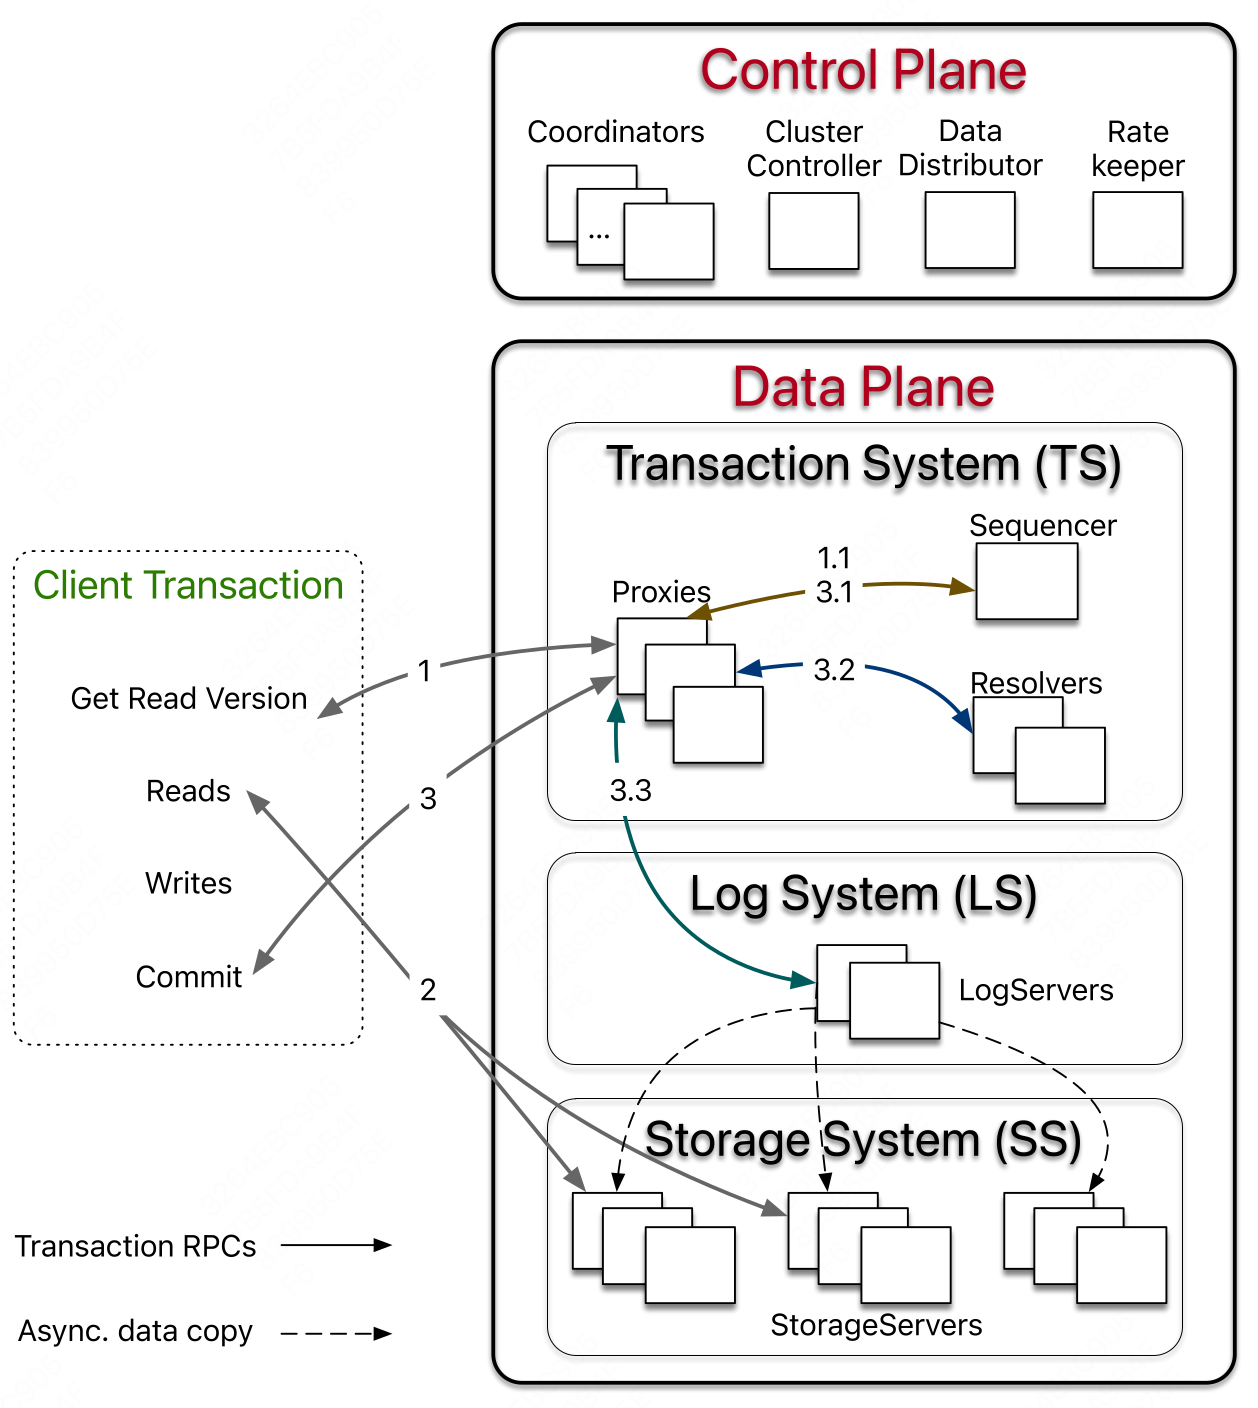
\includegraphics[width=.8\textwidth]{../../images/papers/108.png}
\captionof{figure}{\label{f1}The architecture and the transaction processing of FDB}
\end{center}
\subsubsection{Control Plane}
\label{sec:orgba8185c}
The control plane is responsible for persisting critical system metadata, i.e., the configuration of
transaction systems, on Coordinators. These Coordinators form a disk Paxos group and select a
singleton \texttt{ClusterController}. The \texttt{ClusterController} monitors all servers in the cluster and recruits
three singleton processes, \texttt{Sequencer}, \texttt{DataDistributor}, and \texttt{Ratekeeper}, which are re-recruited if they
fail or crash. The \texttt{Sequencer} assigns read and commit versions to transactions. The \texttt{DataDistributor} is
responsible for monitoring failures and balancing data among \texttt{StorageServers}. \texttt{Ratekeeper} provides
overload protection for the cluster.
\subsubsection{Data Plane}
\label{sec:org45e5fe7}
FDB targets OLTP workloads that are read-mostly, read and write a small set of keys, have low
contention, and require scalability. FDB chooses an unbundled architecture: a distributed transaction
management system (TS) performs in-memory transaction processing, a log system (LS) stores
Write-Ahead-Log (WAL) for TS, and a separate distributed storage system (SS) is used for storing data
and servicing reads. The TS provides transaction processing and consists of a \texttt{Sequencer}, \texttt{Proxies}, and
\texttt{Resolvers}, all of which are stateless processes. The LS contains a set of \texttt{LogServers} and the SS has a
number of \texttt{StorageServers}.

\begin{itemize}
\item The \texttt{Sequencer} assigns a read version and a commit version to each transaction and, for historical
reasons, also recruits \texttt{Proxies}, \texttt{Resolvers}, and \texttt{LogServers}.
\item \texttt{Proxies} offer MVCC read versions to clients and orchestrate transaction commits.
\item \texttt{Resolvers} check for conflicts between transactions.
\item \texttt{LogServers} act as replicated, sharded, distributed persistent queues, where each queue stores WAL
data for a \texttt{StorageServer}.
\end{itemize}


The SS consists of a number of \texttt{StorageServers} for serving client reads, where each \texttt{StorageServer}
stores a set of data shards, i.e., contiguous key ranges. \texttt{StorageServers} are the majority of processes
in the system, and together they form a distributed B-tree. Currently, the storage engine on each
\texttt{StorageServer} is a modified version of SQLite, with enhancements that make range clears faster,
defer deletion to a background task, and add support for asynchronous programming.

\wu{
Why SQLite? Why not RocksDB? Two fold:

\begin{enumerate}
\item According to the \href{https://forums.foundationdb.org/t/rocksdb-backend/845/2}{thread}: They do not work with the simulation testing framework as they require
thread pools because they do synchronous IO. The simulation testing framework requires that every
part of the database be able to run in a single thread.
\item FDB's \href{https://www.youtube.com/watch?v=nlus1Z7TVTI}{scenario} has more range reads. B+ tree outperforms LSM tree.
\end{enumerate}

But in FDB 8.0, rocksdb will be supported. (Guess c++20's coroutine makes this work?)
}
\subsubsection{Read-Write Separation and Scaling}
\label{sec:org2211a22}
FDB’s design is decoupled; processes are assigned different roles (e.g., \texttt{Coordinators}, \texttt{StorageServers},
\texttt{Sequencer}), and the database scales by expanding the number of processes for each role. This separates
the scaling of client reads from client writes (i.e., transaction commits).
\begin{itemize}
\item Because clients directly issue reads to sharded \texttt{StorageServers}, reads scale linearly with the number of \texttt{StorageServers}.
\item Writes are scaled by adding more processes to \texttt{Proxies}, \texttt{Resolvers}, and \texttt{LogServers} in TS and LS. For
this reason, MVCC data is stored in the SS.
\item The singletons (e.g., \texttt{ClusterController} and \texttt{Sequencer}) and \texttt{Coordinators} on the control plane are not
performance bottlenecks, because they only perform limited metadata operations.
\end{itemize}
\subsubsection{Bootstrapping}
\label{sec:org376ebb4}
FDB has no external dependency on other services. All user data and most of the system metadata (keys
that start with \texttt{0xFF} prefix) are stored in \texttt{StorageServers}. The metadata about \texttt{StorageServers} is
persisted in \texttt{LogServers}, and the configuration of LS (i.e., information about \texttt{LogServers}) is stored in
all \texttt{Coordinators}.
\begin{enumerate}
\item Using Coordinators as a disk Paxos group, servers attempt to become the \texttt{ClusterController} if one
does not exist.
\item The newly elected \texttt{ClusterController} recruits a new \texttt{Sequencer}
\item The \texttt{sequencer} reads the configuration of old LS stored in \texttt{Coordinators} and spawns a new TS and LS.
\item From the old LS, \texttt{Proxies} recover system metadata, including information about all \texttt{StorageServers}.
\item The \texttt{Sequencer} waits until the new TS finishes recovery, and then writes the new LS configuration to
all \texttt{Coordinators}.
\end{enumerate}
At this time, the new transaction system becomes ready to accept client transactions.
\subsubsection{Reconfiguration}
\label{sec:org70a421b}
Whenever there is a failure in the TS or LS, or a database configuration change, a reconfiguration
process brings the transaction management system to a new configuration, i.e., a clean state.
Specifically, the \texttt{Sequencer} process monitors the health of \texttt{Proxies}, \texttt{Resolvers}, and \texttt{LogServers}. If any
one of the monitored processes fails or the database configuration changes, the \texttt{Sequencer} process
terminates. The \texttt{ClusterController} will detect the \texttt{Sequencer} failure event, then recruit a new
Sequencer, which follows the above bootstrapping process to spawn the new TS and LS instance. In this
way, transaction processing is divided into epochs, where each epoch represents a generation of the
transaction management system with its unique Sequencer process.
\subsection{Transaction Management}
\label{sec:org36082c0}
\subsubsection{End-to-end Transaction Processing}
\label{sec:org836a7eb}
\begin{enumerate}
\item A client transaction starts by contacting one of the \texttt{Proxies} to obtain a read version (i.e., a
timestamp).
\item The \texttt{Proxy} then asks the \texttt{Sequencer} for a read version that is guaranteed to be no less than any
previously issued transaction commit version, and this read version is sent back to the client.
\item Then the client may issue multiple reads to \texttt{StorageServers} and obtain values at that specific read
version.
\end{enumerate}

Client writes are buffered locally without contacting the cluster. At commit time, the client sends
the transaction data, including the read and write sets (i.e., key ranges), to one of the \texttt{Proxies} and
waits for a commit or abort response from the \texttt{Proxy}. If the transaction cannot commit, the client may
choose to restart the transaction from the beginning again.

A \texttt{Proxy} commits a client transaction in three steps.
\begin{enumerate}
\item The \texttt{Proxy} contacts the \texttt{Sequencer} to obtain a commit version that is larger than any existing read
versions or commit versions. The \texttt{Sequencer} chooses the commit version by advancing it at a rate of
one million versions per second.
\item the \texttt{Proxy} sends the transaction information to range-partitioned \texttt{Resolvers}, which implement FDB’s
optimistic concurrency control by checking for read-write conflicts. If all Resolvers return with
no conflict, the transaction can proceed to the final commit stage. Otherwise, the Proxy marks the
transaction as aborted.
\item committed transactions are sent to a set of \texttt{LogServers} for persistence. A transaction is considered
committed after all designated \texttt{LogServers} have replied to the \texttt{Proxy}, which reports the committed
version to the \texttt{Sequencer} (to ensure that later transactions’ read versions are after this commit)
and then replies to the client. At the same time, \texttt{StorageServers} continuously pull mutation logs
from \texttt{LogServers} and apply committed updates to disks.
\end{enumerate}

In addition to the above read-write transactions, FDB also supports read-only transactions and
snapshot reads. A read-only transaction in FDB is both serializable (happens at the read version) and
performant (thanks to the MVCC), and the client can commit these transactions locally without
contacting the database. This is particularly important because the majority of transactions are
read-only. Snapshot reads in FDB selectively relax the isolation property of a transaction by reducing
conflicts, i.e., concurrent writes will not conflict with snapshot reads.
\subsubsection{Support Strict Serializability}
\label{sec:org3c5523a}
FDB implements Serializable Snapshot Isolation (SSI) by combining OCC with MVCC. Recall that a
transaction \(T_x\) gets both its read version and commit version from \texttt{Sequencer}, where the read
version is guaranteed to be no less than any committed version when \(T_x\) starts and the commit
version is larger than any existing read or commit versions.

This commit version defines a serial history for transactions and serves as Log Sequence Number (LSN).
Because \(T_x\) observes the results of all previous committed transactions, FDB achieves strict
serializability. To ensure there is no gaps between LSNs, the \texttt{Sequencer} returns the previous commit version (i.e., previous LSN) with commit version.

A \texttt{Proxy} sends both LSN and previous LSN to \texttt{Resolvers} and \texttt{LogServers} so that they can serially process
transactions in the order of LSNs. Similarly, \texttt{StorageServers} pull log data from \texttt{LogServers} in
increasing LSNs as well.

\begin{center}
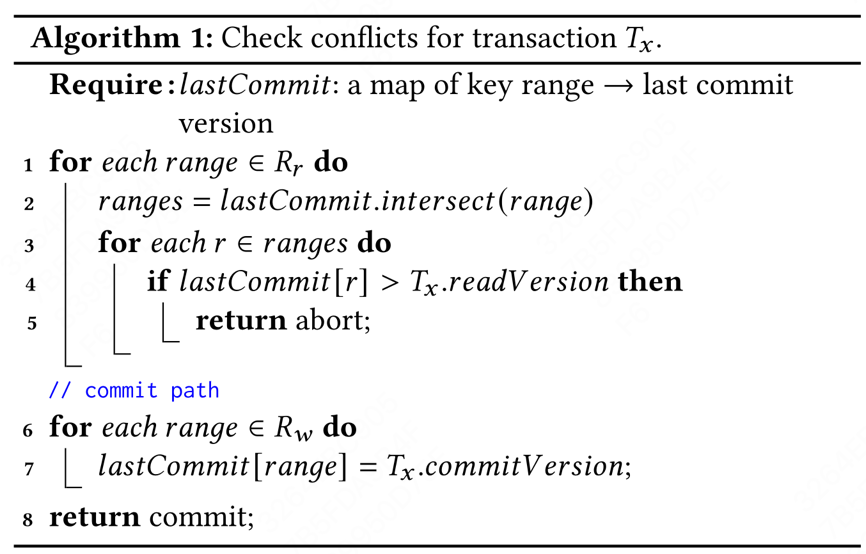
\includegraphics[width=.8\textwidth]{../../images/papers/109.png}
\label{a1}
\end{center}

Algorithm \ref{a1} illustrates the lock-free conflict detection algorithm on \texttt{Resolvers}. Specifically,
each \texttt{Resolver} maintains a history of \(lastCommit\) recently modified key ranges by committed
transactions, and their corresponding commit versions. The commit request for \(T_x\) comprises two
sets: a set of modified key ranges \(R_w\), and a set of read key ranges \(R_r\), where a single key
is converted to a single key range. The read set is checked against the modified key ranges of
concurrent committed transactions (line 1—5), which prevents phantom reads. If there are no read-write
conflicts, \texttt{Resolvers} admit the transaction for commit and update the list of modified key ranges with
the write set (line 6—7). For snapshot reads, they are not included in the set \(R_r\) . In practice,
\(lastCommit\) is represented as a version-augmented probabilistic SkipList.

The entire key space is divided among \texttt{Resolvers} so that the above read-write conflict detection
algorithm may be performed in parallel. A transaction can commit only when all \texttt{Resolvers} admit the
transaction. Otherwise, the transaction is aborted.

It is possible that an aborted transaction is admitted by a subset of \texttt{Resolvers}, and they have already
updated their history of \(lastCommit\), which may cause other transactions to conflict (i.e., a false positive).
In practice, this has not been an issue for our production workloads:
\begin{itemize}
\item transactions’ key ranges usually fall into one Resolver.
\item Additionally, because the modified keys expire after the MVCC window, the false positives are
limited to only happen within the short MVCC window time (i.e., 5 seconds).
\item the key ranges of \texttt{Resolvers} are dynamically adjusted to balance their loads.
\end{itemize}

The OCC design of FDB avoids the complicated logic of acquiring and releasing (logical) locks, which
greatly simplifies interactions between the TS and the SS. The price paid for this simplification is
to keep the recent commit history in \texttt{Resolvers}. Another drawback is not guaranteeing that transactions
will commit, a challenge for OCC. Because of the nature of our multi-tenant production workload, the
transaction conflict rate is very low (less than 1\%) and OCC works well. If a conflict happens, the
client can simply restart the transaction.
\subsubsection{Logging Protocol}
\label{sec:org59305ec}
\begin{center}
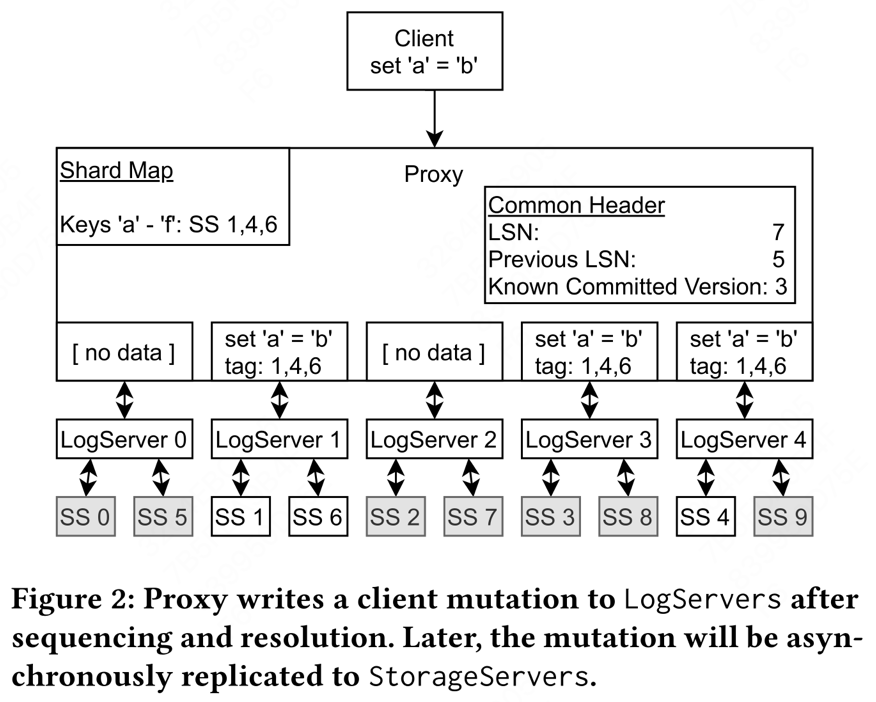
\includegraphics[width=.7\textwidth]{../../images/papers/110.png}
\label{f2}
\end{center}

After a \texttt{Proxy} decides to commit a transaction, the log message is broadcast to all \texttt{LogServers}. As
illustrated in Figure \ref{f2}, the Proxy first consults its in-memory shard map to determine the
\texttt{StorageServers} responsible for the modified key range. Then the Proxy attaches StorageServer tags 1,
4, and 6 to the mutation, where each tag has a preferred LogServer for storage.

In this example, tags 1 and 6 have the same preferred \texttt{LogServer}. Note the mutation is only sent to the
preferred LogServers (1 and 4) and an additional LogServer 3 to meet the replication requirements. All
other \texttt{LogServers} receive an empty message body. The log message header includes both LSN and the
previous LSN obtained from the Sequencer, as well as the known committed version (KCV) of this Proxy.
LogServers reply to the Proxy once the log data is made durable, and the Proxy updates its KCV to the
LSN if all replica LogServers have replied and this LSN is larger than the current KCV.

Shipping the redo log from the LS to the SS is not a part of the commit path and is performed in the
background. In FDB, StorageServers aggressively fetch redo logs from LogServers before they are
durable on the LS, allowing very low latency for serving multi-version reads.

\begin{center}
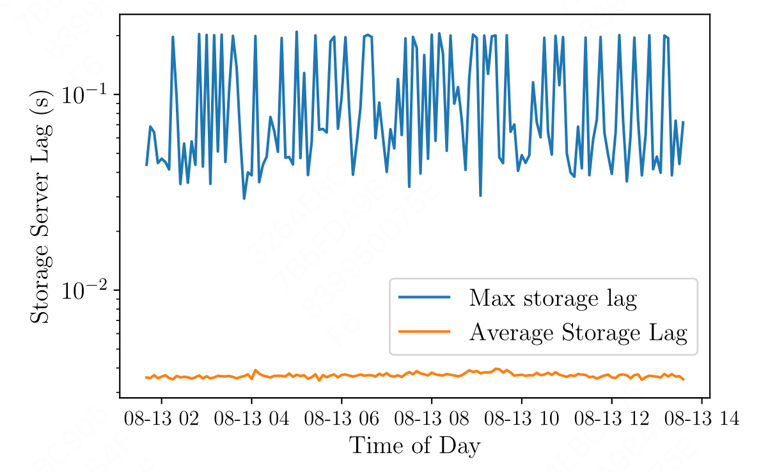
\includegraphics[width=.5\textwidth]{../../images/papers/111.png}
\captionof{figure}{\label{f3}The lag from StorageServers to LogServers}
\end{center}

Figure \ref{f3} shows the time lag between StorageServers and LogServers in one of our production
clusters for a 12-hour period, where the 99.9 percentile of the average and maximum delay is 3.96 ms
and 208.6 ms, respectively. Because this lag is small, when client read requests reach StorageServers,
the requested version (i.e., the latest committed data) is usually already available. If due to a
small delay the data is not available to read at a StorageServer replica, the client either waits for
the data to become available or issues a second request to another replica. If both reads timed out,
the client gets a retryable error to restart the transaction.

Because the log data is already durable on LogServers, StorageServers can buffer updates in memory and
only persist batches of data to disks with a longer delay, thus improving I/O efficiency by coalescing
the updates. Aggressively pulling redo logs from LogServers means that semi-committed updates, i.e.,
operations in transactions that are aborted during recovery (e.g., due to LogServer failure), need to
be rolled back.
\subsubsection{Transaction System Recovery}
\label{sec:org852a0b9}
In FDB, \texttt{StorageServers} always pull logs from \texttt{LogServers} and apply them in the background, which
essentially decouples redo log processing from the recovery. The recovery process starts by detecting
a failure, recruits a new transaction system, and ends when old \texttt{LogServers} are no longer needed. The
new transaction system can even accept transactions before all the data on old \texttt{LogServers} is
processed, because the recovery only needs to find out the end of redo log and re-applying the log is
performed asynchronously by StorageServers.

For each epoch, the \texttt{Sequencer} executes recovery in several steps.
\begin{enumerate}
\item the \texttt{Sequencer} reads the previous transaction system states (i.e. configurations of the transaction
system) from \texttt{Coordinators} and locks the coordinated states to prevent another \texttt{Sequencer} process
from recovering at the same time.
\item the \texttt{Sequencer} recovers previous transaction system states, including the information about all
older \texttt{LogServers}, stops these \texttt{LogServers} from accepting transactions, and recruits a new set of
\texttt{Proxies}, \texttt{Resolvers}, and \texttt{LogServers}.
\item After previous \texttt{LogServers} are stopped and a new transaction system is recruited, the \texttt{Sequencer} then
writes the coordinated states with current transaction system information.
\item Finally, the Sequencer accepts new transaction commits.
\end{enumerate}

Because \texttt{Proxies} and \texttt{Resolvers} are stateless, their recoveries have no extra work. In contrast,
\texttt{LogServers} save the logs of committed transactions, and we need to ensure a ll previously committed
transactions are durable and retrievable by \texttt{StorageServers}. That is, for any transactions that the
\texttt{Proxies} may have sent back a commit response, their logs are persisted in multiple \texttt{LogServers}
satisfying the configured replication degree.

The essence of the recovery of old \texttt{LogServers} is to determine the end of redo log, i.e., a Recovery
Version (RV). Rolling back undo log is essentially discarding any data after RV in the old
\texttt{LogServers} and \texttt{StorageServers}. Figure \ref{f4} illustrates how RV is determined by the Sequencer.
\begin{center}
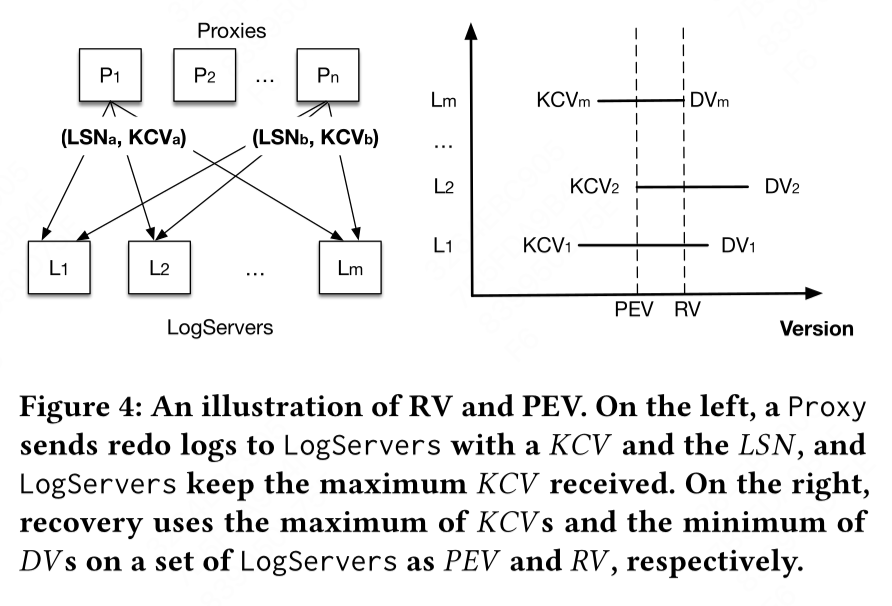
\includegraphics[width=.5\textwidth]{../../images/papers/112.png}
\label{f4}
\end{center}


Recall that a \texttt{Proxy} request to \texttt{LogServers} piggybacks its KCV, the maximum LSN that this Proxy has
committed. Each LogServer keeps the maximum KCV received and a Durable Version (DV), which is the
maximum persisted LSN. During a recovery, the \texttt{Sequencer} attempts to stop all \(m\) old \texttt{LogServers},
where each response contains the DV and KCV on that \texttt{LogServer}. Assume the replication degree for
LogServers is \(k\). Once the \texttt{Sequencer} has received more than \(m-k\) replies , the \texttt{Sequencer} knows
the previous epoch has committed transactions up to the maximum of all KCVs, which becomes the
previous epoch’s end version (PEV). All data before this version has been fully replicated.

For current epoch, its start version is PEV+1 and the \texttt{Sequencer} chooses the minimum of all DVs to be
the RV. Logs in the range of \([PEV+1,RV]\) are copied from previous epoch’s \texttt{LogServers} to the current
ones, for healing the replication degree in case of \texttt{LogServer} failures. The overhead of copying this
range is very small because it only contains a few seconds’ log data.

When \texttt{Sequencer} accepts new transactions, the first is a special recovery transaction that informs
\texttt{StorageServers} the RV so that they can roll back any data larger than RV. The current FDB storage
engine consists of an unversioned SQLite B-tree and in-memory multi-versioned redo log data. Only
mutations leaving the MVCC window (i.e., committed data) are written to SQLite. The rollback is simply
discarding in-memory multi-versioned data in \texttt{StorageServers}. Then \texttt{StorageServers} pull any data larger
than version \(PEV\) from new \texttt{LogServers}.
\subsection{Replication}
\label{sec:org6138ef9}
FDB uses a combination of various replication strategies for differ ent data to tolerate \(f\)
failures:
\begin{itemize}
\item \emph{Metadata replication}. System metadata of the control plane is stored on Coordinators using Active
Disk Paxos. As long as a quorum (i.e., majority) of Coordinators are live, this metadata can be
recovered.
\wu{Why choose this version of Paxos?}
\item \emph{Log replication}. When a Proxy writes logs to LogServers, each sharded log record is synchronously
replicated on \(k=f+1\) \texttt{LogServers}. Only when all \(k\) have replied with successful persistence can
the Proxy send back the commit response to the client. Failure of a LogServer results in a
transaction system recovery.
\item \emph{Storage replication}. Every shard, i.e., a key range, is asynchronously replicated to \(k=f+1\)
StorageServers, which is called a \textbf{team}. A \texttt{StorageServer} usually hosts a number of shards so that its
data is evenly distributed across many teams. A failure of a \texttt{StorageServer} triggers \texttt{DataDistributor}
to move data from teams containing the failed process to other healthy teams
\end{itemize}


\wu{
Why do FoundationDB need to consider this?

What if we want to split the storage server
}


Note the storage team abstraction is more sophisticated than the Copyset policy. Copyset reduces the
chance of data loss during simultaneous process failures by assigning shards to a limited number of
possible \(k\)-process groups. Otherwise, any \(k\)-process failure can cause a higher probability of
data loss. In our deployment, teams need to consider multiple dimensions: each replica group needs to
satisfy several constraints at the same time. For instance, a cluster can have a number of hosts and
each host runs multiple processes. In this case, a failure can happen at the host level, affecting
many processes. Thus, a replica group cannot place two processes on the same host. More generally, the
placement needs to ensure at most one process in a replica group can be placed in a fault domain,
e.g., racks or availability zones in a cloud environment.

To solve the above problem, we designed a hierarchical replication policy to reduce the chance of data
loss during simultaneous failures. Specifically, we construct the replica set at both host and process
levels and ensure that each process group belongs to a host group that satisfies the fault domain
requirement. This policy has the benefits that data loss can only happen when all hosts in a selected
host group fail simultaneously; that is, when we experience concurrent failures in multiple fault
domains. Otherwise, each team is guaranteed to have at least one process live and there is no data
loss if any one of the fault domains remains available..
\subsection{Other Optimizations}
\label{sec:org5878f0d}
\begin{itemize}
\item \textbf{Transaction batching}
\item \textbf{Atomic operations}. FDB supports atomic operations such as atomic add, bitwise “and” operation,
compare-and-clear, and set-versionstamp.
\end{itemize}
\section{Geo-replication and failover}
\label{sec:org14e5b31}
The main challenge of providing high availability during region failures is the trade-off of
performance and consistency. Synchronous cross-region replication provides strong consistency, but
pays the cost of high latency. Conversely, asynchronous replication reduces latency by only persisting
in the primary region, but may lose data when performing a region failover. FDB can be configured to
perform either synchronous or asynchronous cross-region replication. However, there is a third
possibility that leverages multiple availability zones within the same region, and provides a high
level of failure independence, notwithstanding the unlikely event of a complete region outage.

Our design
\begin{enumerate}
\item always avoids cross-region write latencies, as for asynchronous replication
\item provides full transaction durability, like synchronous replication, so long as there is no
simultaneous failure of multiple availability zones in a region,
\item can do rapid and completely automatic failover between regions,
\item can be manually failed-over with the same guarantees as asynchronous replication (providing A, C,
and I of ACID but potentially exhibiting a Durability failure) in the unlikely case of a
simultaneous total region failure
\item only requires full replicas of the database in the primary and secondary regions’ main availability
zones, not multiple replicas per region. The rest of this section is dedicated to this design.
\end{enumerate}
\begin{center}
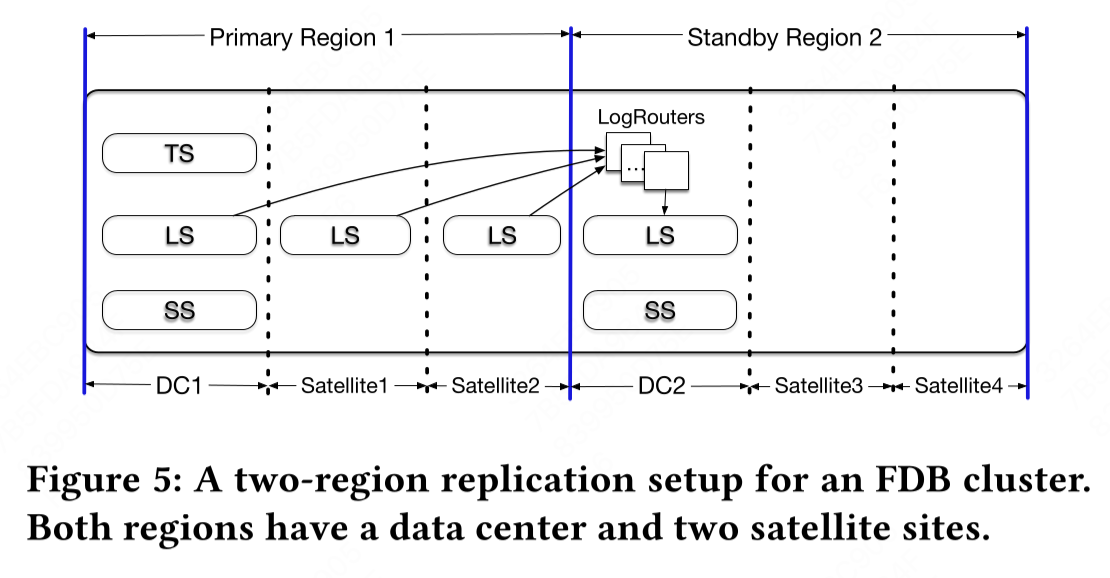
\includegraphics[width=.6\textwidth]{../../images/papers/113.png}
\label{f5}
\end{center}

Figure \ref{f5} illustrates the layout of a two-region replication of a cluster. Both regions have a
data center (DC) as well as one or more satellite sites. Satellites are located in close proximity to
the DC (in the same region) but are failure independent. The resource requirements from satellites are
insignificant as they only need to store log replicas (i.e., a suffix of the redo logs), while data
centers host LS, SS, and (when primary) the TS. Control plane replicas (i.e., coordinators) are
deployed across three or more failure domains (in some deployments utilizing an additional region),
usually with at least 9 replicas. Relying on majority quorums allows the control plane to tolerate one
site (data center/satellite) failure and an additional replica failure.

A typical deployment configuration is illustrated in Figure \ref{f5}, depicting two regions with a data
center and two satellites in each region.
\begin{itemize}
\item One of the data centers (DC1), configured with a higher priority compared to DC2, is designated as
the primary (its region is denoted as the primary region, accordingly) and contains the full TS, LS,
and SS
\item DC2 in the secondary region has replicas of data with its own LS and SS
\item Reads can be served from storage replicas at both primary and secondary data centers (consistent
reads do require obtaining a read version from the primary data center).
\item All client writes are forwarded to the primary region and processed by Proxies in DC1, then
synchronously persisted onto LogServers in DC1 and one or both satellite sites in the primary region
(depending on the configuration), avoiding the cross-region WAN latency.

The updates are then asynchronously replicated to DC2, where they are stored on multiple LS servers
and eventually spread out to multiple StorageServers.
\item LogRouters implement a special type of FDB role that facilitates cross-region data transfer. They
were created to avoid redundant cross-region transfers of the same information. Instead, LogRouters
transfer each log entry across WAN only once, and then deliver it to all relevant LS servers locally in DC2.
\end{itemize}


\begin{itemize}
\item The cluster automatically fails-over to the secondary region if the primary data center becomes
unavailable. Satellite failures could, in some cases, also result in a fail-over, but this decision
is currently manual.
\item When the fail-over happens, DC2 might not have a suffix of the log, which it proceeds to recover
from the remaining log server in the primary region.
\end{itemize}

Next, we discuss several alternative satellite configurations which provide different levels of
fault-tolerance. Satellite configuration can be specified per region. Each satellite is given a static
priority, which is considered relatively to other satellites in the same region. FDB is usually
configured to store multiple log replicas at each location. Three main alternatives are supported:
\begin{enumerate}
\item synchronously storing updates on all log replicas at the satellite with the highest priority in the
region. In this case, if the satellite fails, another satellite with the next priority is recruited
for the task
\item synchronously storing updates on all replicas of two satellites with the highest priorities in the
region. In this case, if a satellite fails, it can be similarly replaced with a different satellite
of lower priority, or, if none available, fall back to option (1) of using a single satellite. In
either case, the secondary region isn’t impacted, as it can continue to pull updates from remaining
LogServers in the primary region.
\item Similar to option (2) but FDB only waits for one of the two satellites to make the mutations
durable before considering a commit successful.
\end{enumerate}

In all cases, if no satellites are available, only the LogServers in DC1 are used. With option 1 and
3, a single site (data center or satellite) failure can be tolerated, in addition to one or more
LogServer failures (since the remaining locations have multiple log replicas). With option 2, two site
failures in addition to one or more LogServer failures can be tolerated. In options 1 and 2, however,
commit latency is sensitive to the tail network latencies between the primary data center and its
satellites, which means that option 3 is usually faster. The choice ultimately depends on the number
of available satellite locations, their connectivity to the data center and the desired level of fault
tolerance and availability.

When DC1 in the primary region suddenly becomes unavailable, the cluster (with the help of
Coordinators) detects the failure and starts a new transaction management system in DC2. New
LogServers are recruited from satellites in the secondary region, in accordance with the region’s
replication policy. During recovery, LogRouters in DC2 may need to fetch the last few seconds’ data
from primary satellites, which, due to the asynchronous replication, may not have made it to DC2 prior
to the failover. After the recovery, if the failures in Region 1 are healed and its replication policy
can again be met, the cluster will automatically fail-back to have DC1 as the primary data center due
to its higher priority. Alternatively, a different secondary region can be recruited.
\section{Simulation Testing}
\label{sec:org1f668be}
\begin{center}
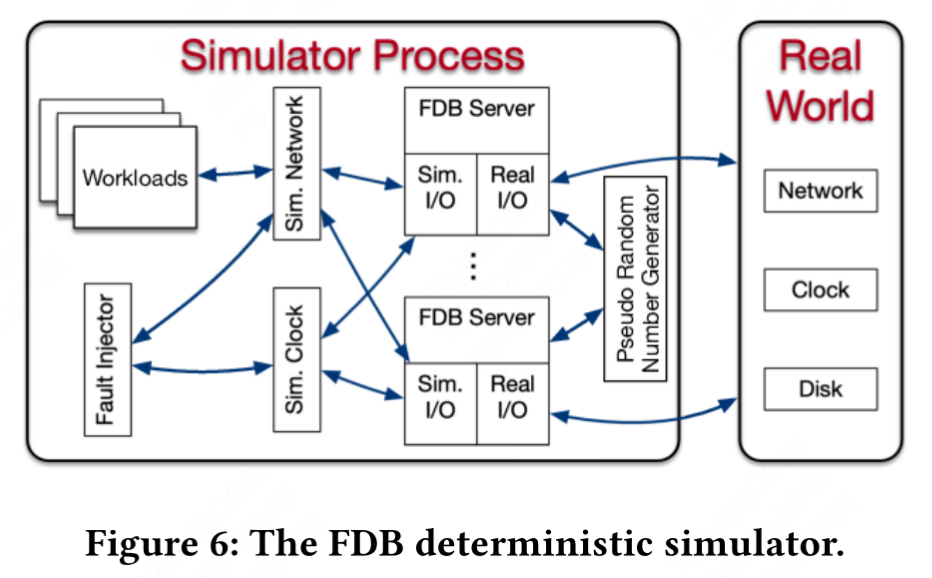
\includegraphics[width=.5\textwidth]{../../images/papers/114.png}
\label{f6}
\end{center}

\begin{itemize}
\item \textbf{Deterministic simulator}. FDB was built from the ground up to make this testing approach possible.
All database code is deterministic; accordingly multithreaded concurrency is avoided (instead, one
database node is deployed per core). Figure \ref{f6} illustrates the simulator process of FDB, where
all sources of nondeterminism and communication are abstracted, including network, disk, time, and
pseudo random number generator.

FDB is written in Flow, a novel syntactic extension to C++ adding async/await-like concurrency
primitives. Flow provides the Actor programming model that abstracts various actions of the FDB
server process into a number of actors that are scheduled by the Flow runtime library.

The simulator process is able to spawn multiple FDB servers that communicate with each other through
a simulated network in a single discrete-event simulation. The production implementation is a simple
shim to the relevant system calls.

The simulator runs multiple workloads (also written in Flow) that communicate with simulated FDB
servers through the simulated network. These workloads include fault injection instructions, mock
applications, database configuration changes, and direct internal database functionality
invocations. Workloads are composable to exercise various features and are reused to construct
comprehensive test cases.
\end{itemize}
\section{Problems}
\label{sec:org8b43421}


\section{References}
\label{sec:orge9068a7}
\label{bibliographystyle link}
\bibliographystyle{alpha}

\bibliography{/Users/wu/notes/notes/references.bib}
\end{document}
